%% This document is created by
%%  Dr. Putu Harry Gunawan
%% Template untuk Proposal TA 1 dan TA
%% Template ini digunakan untuk penulisan proposal TA 1 atau TA Fakultas Informatika, Telkom University.
%%  New Update 28 Pebruari 2017 : Bookmarks pdf, Pembimbing hanya satu

\documentclass[a4paper,12pt,oneside]{book}
\usepackage[utf8]{inputenc}
\usepackage{sectsty}
\usepackage{graphicx}
\usepackage{epstopdf}
\usepackage{algorithm}
\usepackage{algpseudocode}
\usepackage{array}
\usepackage[table]{xcolor}
\usepackage{anysize}
\usepackage{amsmath}
\usepackage{amssymb}
\usepackage[indonesian]{babel}
\usepackage{indentfirst} %Spasi untuk paragraf pertama
\usepackage{geometry}
\usepackage{multirow}% http://ctan.org/pkg/multirow
\usepackage{hhline}% http://ctan.org/pkg/hhline
\marginsize{4cm}{3cm}{3cm}{3cm} %{left}{right}{top}{bottom}
\usepackage[compact]{titlesec}
\usepackage{etoolbox}
\usepackage[numbers]{natbib} %for numbered citations with unsrt
\usepackage[bookmarks,hypertexnames=false,debug]{hyperref}
%\usepackage[pageanchor]{hyperref}
\usepackage{bookmark}
% untuk tabel yang panjang
\usepackage{longtable}
\usepackage{array}
\usepackage{caption}
% untuk rata kanan kiri
\usepackage{microtype}


\makeatletter
\patchcmd{\ttlh@hang}{\parindent\z@}{\parindent\z@\leavevmode}{}{}
\patchcmd{\ttlh@hang}{\noindent}{}{}{}
\makeatother

\chapterfont{\centering}
\newcommand{\bigsize}{\fontsize{16pt}{14pt}\selectfont}
\chapterfont{\centering\bigsize\bfseries}
\sectionfont{\large\bfseries}
\usepackage{tikz}
\usetikzlibrary{shapes.geometric, arrows}
%\renewcommand{\chaptertitle}{BAB}
\renewcommand{\thechapter}{\Roman{chapter}}
\renewcommand\thesection{\arabic{chapter}.\arabic{section}}
\renewcommand\thesubsection{\thesection.\arabic{subsection}}
\renewcommand{\theequation}{\arabic{chapter}.\arabic{equation}}
\renewcommand{\thefigure}{\arabic{chapter}.\arabic{figure}}
\renewcommand{\thetable}{\arabic{chapter}.\arabic{table}}

\renewcommand\bibname{Daftar Pustaka}
\addto{\captionsbahasa}{\renewcommand{\bibname}{Daftar Pustaka}}
\usepackage{fancyhdr}
\pagestyle{fancy}
\lhead{}
\chead{}
\rhead{}
\lfoot{}
\cfoot{\thepage}
\rfoot{}
\renewcommand{\headrulewidth}{0pt}

\makeatletter

%%%%%%%%%%%%%%%%%%%%%%%%%%%%%%%%%%%%%%%%%%%%%%%%%%%%%%%%%%%%
%
%  Berikut adalah data-data yang wajib diisi oleh mahasiswa
%
%%%%%%%%%%%%%%%%%%%%%%%%%%%%%%%%%%%%%%%%%%%%%%%%%%%%%%%%%%%%

\title{Evaluasi Komparatif dan Uji Generalisasi Arsitektur \textit{Deep Learning} untuk Deteksi Kerusakan dan Cacat Permukaan Jalan di Indonesia}\let\Title\@title

\newcommand{\EngTitle}{Comparative Evaluation and Generalization Testing of Deep Learning Architectures for Road Damage and Surface Defect Detection in Indonesia}

% Opsi 2
% \title{Evaluasi Komparatif dan Analisis \textit{Domain Gap} Arsitektur \textit{Deep Learning} untuk Deteksi Kerusakan Jalan Raya di Indonesia}\let\Title\@title

% \newcommand{\EngTitle}{Comparative Evaluation and Domain Gap Analysis of Deep Learning Architectures for Road Damage Detection in Indonesia}

% Opsi 3
% \title{Evaluasi Komparatif Arsitektur \textit{Deep Learning} untuk Deteksi Kerusakan Jalan Lintas Domain pada Perangkat Terbatas di Indonesia}\let\Title\@title

% \newcommand{\EngTitle}{Comparative Evaluation of Deep Learning Architectures for Cross-Domain Road Damage Detection on Constrained Devices in Indonesia}




\author{Faaris Khairrudin}  \let\Author\@author  %Nama mhs
\newcommand{\NIM}{103052300115}
\newcommand{\Prodi}{Sains Data}
\newcommand{\KK}{Modelling Computational Experiment} %UNTUK TA
\newcommand{\Gelar}{Sains Komputasi} % UNTUK TA
\date{2026}           \let\Date\@date %Masukkan hanya tahun saja
\newcommand{\Tanggal}{4} % Tanggal Pengesahan
\newcommand{\Bulan}{September} % Bulan Pengesahan
\newcommand{\PembimbingSatu}{Dr. GAMMA KOSALA, S.Si}
\newcommand{\NIPPembimbingSatu}{26920005}
\newcommand{\PembimbingDua}{Dr. Calon Pembimbing 2, M.Kom}
\newcommand{\NIPPembimbingDua}{123456}
\newcommand{\Kaprodi}{Dr. GAMMA KOSALA, S.Si}
\newcommand{\NIPKaprodi}{26920005}
\newif\ifPembimbingHanyaSatu

%%%% WARNING kode berikut ini diaktifkan Jika pembimbing hanya satu %%%%

\PembimbingHanyaSatutrue

%%%%%%%%%%%%%%%%%%%%%%%%%%%%%%%%%%%%%%%%%%%%%%%%%%%%%%%%%%%%%%%%%%

\makeatother
\linespread{1}


\begin{document}
%%%%%%%%%%%%%%%%%%%%%%%%%%%%%%%%%%%%%%%%%%%%%%%%%%%%%%%%%%
% Dimulai dengan cover, lembar persetujuan, Abstrak, dll
%%%%%%%%%%%%%%%%%%%%%%%%%%%%%%%%%%%%%%%%%%%%%%%%%%%%%%%%%%%
\pagenumbering{roman}
\begin{titlepage}
  \thispagestyle{empty}
  %\vspace*{0.7cm}
  \pdfbookmark{Cover}{cover}
  \include{Cover}
  \pagebreak
  \thispagestyle{empty}
  \pdfbookmark{Lembar Persetujuan}{lembar-persetujuan}
  \include{Lembar-Persetujuan}
  \pagebreak
\end{titlepage}
\phantomsection
\addcontentsline{toc}{chapter}{Abstrak}
%\pdfbookmark{\abstractname}{Abstrak Indonesia}
\chapter*{Abstrak}
Infrastruktur jalan yang memadai merupakan prasyarat krusial bagi mobilitas ekonomi dan keselamatan transportasi. Inspeksi kerusakan jalan secara manual dinilai tidak efisien, padat karya, dan rentan terhadap subjektivitas. Meskipun algoritma \textit{deep learning} dari keluarga YOLO telah terbukti efektif dalam otomasi deteksi kerusakan jalan, penerapannya di lapangan dihadapkan pada tantangan kesalahan deteksi (\textit{false positive}) akibat objek pengecoh visual (seperti penutup saluran air dan jalan bertambal), serta kebutuhan efisiensi komputasi tinggi pada perangkat terbatas untuk pengawasan waktu nyata (\textit{real-time}).

Penelitian ini melakukan evaluasi komparatif terhadap lima arsitektur deteksi objek berskala nano (`n'): YOLOv8n (\textit{baseline}), arsitektur mutakhir (YOLOv12n dan YOLOv26n), serta dua model rekonstruksi modifikasi domain-spesifik, yaitu YOLOv8-PD (\textit{efficiency-oriented}) dan YOLO-RD (\textit{accuracy-oriented}). Seluruh model dilatih menggunakan dataset N-RDD2024 subset Asia (enam kelas target: empat kerusakan struktural dan dua objek pengecoh) dengan skema pembobotan teradaptasi \textit{Effective Number of Samples} untuk menangani ketimpangan kelas. Kinerja deteksi dievaluasi menggunakan metrik mAP@0.5, mAP@0.5:0.95, dan \textit{macro F1}, sedangkan kelayakan komputasi dianalisis berdasarkan jumlah parameter, GFLOPs, dan kecepatan inferensi (FPS) pada GPU NVIDIA RTX 4070 SUPER. Selain itu, dilakukan studi ablasi pemodelan 6-kelas versus 4-kelas untuk menguji hipotesis penekanan \textit{false positive} menggunakan uji signifikansi statistik \textit{two-proportion z-test}.

Hasil eksperimen membuktikan konfirmasi filosofi desain masing-masing arsitektur. Model rekonstruksi YOLO-RD berhasil meraih akurasi tertinggi dengan nilai test mAP@0.5 sebesar 0,661 dan test mAP@0.5:0.95 sebesar 0,371, membuktikan keunggulan integrasi atensi deformabel dan dekomposisi Haar wavelet. Sementara itu, YOLOv8-PD terbukti paling efisien dengan bobot teringan (2,46M parameter) dan kecepatan inferensi tertinggi mencapai 368,4 FPS (+67,7\% lebih cepat dari baseline) dengan akurasi setara baseline (0,646 vs. 0,648). Uji statistik ablasi pengecoh menunjukkan perbedaan laju \textit{false positive} yang belum signifikan ($p > 0,05$), di mana penambahan kelas pengecoh memperketat batas keputusan visual yang sedikit menekan mAP lubang jalan (\textit{pothole}) namun meningkatkan keseimbangan skor F1 secara agregat. Temuan ini memberikan panduan empiris yang komprehensif dalam pemilihan arsitektur deteksi kerusakan jalan untuk skenario implementasi praktis.

\vspace{1em}
\textbf{Kata Kunci:} Deteksi Kerusakan Jalan, YOLO, Kelas Pengecoh, Rekonstruksi Arsitektur, N-RDD2024, \textit{Lightweight Model}, Efisiensi Komputasi.

\cleardoublepage
\phantomsection
\addcontentsline{toc}{chapter}{Daftar Isi}
%\pdfbookmark{\contentsname}{Contents}
\tableofcontents

%%%%%%%%%%%%%%%%%%%%%%%%%%%%%%%%%%%%%%%%%%%%%%%%%
% Bab bab penulisan
%%%%%%%%%%%%%%%%%%%%%%%%%%%%%%%%%%%%%%%%%%%%%%%%
\cleardoublepage
\pagenumbering{arabic}
\chapter{Pendahuluan}
\section{Latar Belakang}

Infrastruktur jalan merupakan fondasi utama pengembangan ekonomi dan mobilitas suatu bangsa.
Kondisi jaringan jalan yang baik menjadi prasyarat bagi urbanisasi, pertumbuhan industri,
dan pemenuhan kebutuhan transportasi masyarakat \cite{Zeng2024, radopoulou2015detection}.
Namun, seiring dengan meningkatnya beban lalu lintas dan paparan faktor lingkungan,
kerusakan jalan berupa retak dan lubang tidak hanya menurunkan efisiensi
perjalanan, tetapi juga meningkatkan risiko kecelakaan dan mengancam keselamatan pengemudi
maupun penumpang \cite{Li2024}.

Persoalan kerusakan jalan memiliki dimensi yang lebih kritis di Indonesia.
Hugo dkk. mencatat bahwa penyebab utama kerusakan jalan di
Indonesia meliputi kendaraan yang melebihi batas muatan, kondisi iklim
tropis dengan curah hujan tinggi, drainase jalan yang buruk, kondisi tanah
yang tidak stabil, serta kualitas material perkerasan yang tidak memadai
\cite{hugo2025efficientdet}. Akibatnya, Indonesia secara konsisten
menghadapi kecelakaan lalu lintas, kemacetan berkepanjangan, dan kerusakan
kendaraan yang berkaitan langsung dengan kondisi jalan yang rusak
\cite{hugo2025efficientdet}. Kusumah dkk. menunjukkan bahwa kerusakan
jalan yang parah memaksa pengemudi untuk lebih waspada, dan kondisi ini secara langsung
berpotensi menimbulkan kecelakaan serta tabrakan antar kendaraan di jalan raya Indonesia
\cite{kusumah2023deep}.

Secara tradisional, pemantauan kondisi jalan dilakukan melalui inspeksi manual menggunakan
patroli kendaraan, pencatatan foto, serta tenaga pengawas lapangan. Metode ini dinilai tidak
efisien, membutuhkan sumber daya yang besar, dan rentan terhadap subjektivitas penilaian
\cite{Li2024}. Hosseini dan Smadi menegaskan bahwa tingkat akurasi prediksi kondisi jalan
secara langsung memengaruhi proses pengambilan keputusan dalam sistem manajemen pemeliharaan
infrastruktur \cite{hosseini2021prediction}. Selain itu, selama proses inspeksi berlangsung,
kendaraan patroli dan petugas sering kali harus menduduki badan jalan sehingga berpotensi
menimbulkan kemacetan dan risiko keselamatan tambahan \cite{Li2024}. Hugo dkk.
juga menekankan bahwa metode konvensional ini bersifat \textit{labor-intensive}, berbiaya
tinggi, dan tidak memiliki skalabilitas yang memadai untuk mencakup jaringan jalan nasional
yang luas \cite{hugo2025efficientdet}.

Perkembangan pesat \textit{deep learning} dalam dekade terakhir telah membuka peluang baru
untuk otomasi deteksi kerusakan jalan. Berbeda dengan metode tradisional yang bergantung pada
ekstraksi fitur manual, algoritma \textit{deep learning} mampu secara otomatis mengidentifikasi
lokasi, jenis, dan batas kerusakan dalam citra secara cepat dan akurat \cite{Zeng2024}.
Mandal dkk. melakukan analisis komparatif terhadap berbagai kerangka
\textit{deep learning} untuk klasifikasi distres perkerasan, menemukan bahwa arsitektur
YOLO mencapai F1-\textit{Score} tertinggi sebesar 0,5814 dan 0,5751 pada dua dataset
pengujian yang berbeda, melampaui CenterNet dan EfficientDet \cite{mandal2020deep}.
Sejalan dengan temuan tersebut, berbagai varian arsitektur berbasis YOLO telah dikembangkan khusus untuk
deteksi kerusakan jalan, termasuk RDD-YOLO \cite{Li2024}, YOLOv8-PD \cite{Zeng2024},
YOLO-RD \cite{Wang2025}, YOLO-LWD \cite{Shi_2026}, dan YOLO-LWNet \cite{Wu2023},
yang masing-masing mengusulkan modifikasi arsitektur untuk meningkatkan presisi dan efisiensi
komputasi.

Pengembangan model-model tersebut sebagian besar mengandalkan \textit{Road Damage Dataset
  2022} (RDD2022), sebuah dataset \textit{benchmark} multi-nasional yang dikembangkan oleh
Arya dkk. melalui \textit{Crowdsensing-based Road Damage Detection Challenge}
(CRDDC2022). Dataset ini terdiri atas 47.420 citra jalan dari enam negara (Jepang, India,
Ceko, Norwegia, Amerika Serikat, dan China), dengan lebih dari 55.000 instans anotasi
\textit{bounding box} yang mencakup empat kelas kerusakan struktural: retak memanjang (D00),
retak melintang (D10), retak buaya (D20), dan lubang jalan (D40) \cite{Arya2024846}. Pada
kompetisi CRDDC2022, model terbaik berhasil mencapai F1-\textit{Score} sebesar 0,770 untuk
keenam negara secara agregat, dengan performa terbaik pada dataset Amerika Serikat
(F1~=~0,844) \cite{Arya2024846}.

Namun, di balik capaian tersebut, terdapat dua kesenjangan (\textit{research gap}) yang signifikan. Pertama, masalah \textit{domain shift}: model yang dilatih pada data dari satu negara mengalami degradasi performa yang nyata saat diuji pada data dari negara lain, suatu fenomena yang telah dilaporkan sejak RDD2019 dan dikonfirmasi kembali pada CRDDC2022 \cite{Arya2024846}. Fakta ini menjadi sangat relevan bagi Indonesia, yang sama sekali tidak terwakili dalam RDD2022. Hugo dkk. melaporkan bahwa penerapan EfficientDet-D0 yang dilatih pada data jalan Indonesia dengan 3.321 citra hanya mampu mencapai F1-\textit{Score} terbaik sebesar 59{,}7\%, yang mereka kaitkan dengan kompleksitas fitur visual kerusakan jalan lokal dan tantangan generalisasi pada data yang belum pernah dilihat (\textit{unseen data}) \cite{hugo2025efficientdet}.
% Arya dkk. melalui studi
% \textit{transfer learning} juga menunjukkan bahwa penambahan data dari negara-negara
% tambahan secara substansial meningkatkan kemampuan generalisasi model, sekaligus
% menggarisbawahi pentingnya kehadiran data lokal dalam proses pelatihan \cite{arya2021deep}.

Kedua, terdapat masalah \textit{false positive} yang bersumber dari elemen
permukaan jalan non-kerusakan yang memiliki kemiripan visual tinggi dengan
kerusakan struktural. Matouq dkk. menyatakan secara eksplisit
bahwa mayoritas algoritma berbasis citra yang berfokus pada deteksi lubang
jalan gagal mempertimbangkan secara memadai kemiripan visual
antara \textit{pothole}, \textit{manhole}, dan \textit{patch}, serta
menegaskan adanya kebutuhan mendesak akan dataset pelatihan dan metodologi
yang lebih baik untuk mengatasi tantangan ini secara efektif
\cite{matouq2024ai, Shi_2026}. Konsekuensinya tercermin pada hasil Zeng
dan Zhong, yang menemukan bahwa akurasi deteksi kelas D40
(\textit{pothole}) pada YOLOv8-PD hanya mencapai 53,1\% dan mengakibatkan
\textit{missed detection} yang berulang \cite{Zeng2024}. Rendahnya performa
pada kelas lubang jalan ini merupakan masalah sistemik yang disebabkan oleh
karakteristik objeknya yang tidak beraturan, ukurannya yang kecil, serta
minimnya jumlah sampel latih jika dibandingkan dengan kelas kerusakan lain
\cite{Zeng2024}. Sejalan dengan itu, Kaya dan \c{C}odur mempublikasikan
dataset N-RDD2024, sebuah versi perluasan dari RDD2022 yang mempertahankan
keenam negara asal tetapi memperluas cakupan anotasi menjadi 10 kelas cacat
permukaan, meliputi retak yang telah diperbaiki (D30), penurunan visibilitas
penyeberangan pejalan kaki (D50), penurunan visibilitas marka lajur (D60),
penutup saluran air (\textit{manhole cover}) (D70), segmen jalan yang ditambal (\textit{patchy
  road}, D80), dan \textit{rutting} (D90) \cite{kaya2024nrdd2024}. Dalam
konteks penelitian ini, kelas D70 dan D80 secara khusus diadopsi sebagai
kelas pengecoh (\textit{distractor classes}) selama pelatihan, mengacu pada
temuan Matouq dkk. yang mengidentifikasi keduanya sebagai sumber
utama \textit{false positive} \cite{matouq2024ai}.

Berdasarkan tinjauan terhadap kondisi penelitian yang ada, terdapat celah yang belum terjawab: belum ada studi yang secara sistematis mengevaluasi dan membandingkan performa berbagai arsitektur \textit{deep learning} menggunakan dataset N-RDD2024 dengan anotasi kelas pengecoh (kelas D70 dan D80), sekaligus mengukur secara eksplisit \textit{domain gap} yang terjadi ketika model tersebut diuji pada kondisi jalan nyata di Indonesia melalui evaluasi \textit{zero-shot}. Hal ini menjadi sangat krusial mengingat karakteristik jalan Indonesia seperti tekstur aspal, pola retak, dan distribusi infrastruktur permukaan jalan (seperti penutup saluran dan tambalan) memiliki keunikan lokal yang secara langsung memengaruhi performa model yang dilatih pada dataset global  \cite{Arya2024846, hugo2025efficientdet}. Oleh karena itu, penelitian ini dirancang untuk mengisi kesenjangan tersebut melalui analisis komparatif arsitektur \textit{deep learning} secara terstruktur dengan mengintegrasikan kelas pengecoh dari N-RDD2024 dan menerapkan optimasi fungsi \textit{loss} untuk mengatasi ketimpangan distribusi kelas. Lebih lanjut, penelitian ini juga akan mengukur \textit{generalization gap} ke domain jalan Indonesia secara kuantitatif, serta mengevaluasi \textit{trade-off} antara akurasi dan efisiensi komputasi guna memastikan kelayakannya untuk diimplementasikan pada perangkat komputasi terbatas.

\section{Rumusan Masalah}
Berdasarkan latar belakang yang telah diuraikan, rumusan masalah dirumuskan ke dalam pertanyaan berikut:
\begin{enumerate}
  \item Bagaimana performa deteksi model \textit{deep learning} ketika dilatih menggunakan dataset N-RDD2024 yang memuat kelas kerusakan dan kelas pengecoh?
  \item Bagaimana performa dan kelayakan model untuk skenario \textit{real-time} pada perangkat komputasi terbatas ditinjau dari efisiensi komputasi?
  \item Bagaimana tingkat \textit{domain gap} atau kemampuan generalisasi model terbaik yang dilatih menggunakan dataset global N-RDD2024 ketika diuji secara langsung (\textit{zero-shot}) pada dataset primer kondisi jalan raya nyata di Indonesia?
\end{enumerate}


\section{Tujuan Penelitian}
Sejalan dengan rumusan masalah di atas, tujuan dari penelitian ini dirancang secara berkesinambungan untuk mencapai target berikut:
\begin{enumerate}
  \item Mengevaluasi dan membandingkan performa deteksi dari arsitektur YOLO \textit{baseline}, YOLO modifikasi, dan YOLO terbaru dengan melatihnya menggunakan dataset global N-RDD2024. Evaluasi ini dilakukan untuk mengukur tingkat akurasi (mAP) setiap arsitektur dalam mengenali kelas kerusakan jalan utama, sekaligus menganalisis ketangguhannya dalam menekan tingkat kesalahan deteksi (\textit{false positive}) yang dipicu oleh kemiripan visual dengan objek pengecoh (seperti penutup saluran air dan tambalan jalan).

  \item Menganalisis kelayakan implementasi \textit{real-time} dan efisiensi komputasi dari model yang telah dilatih dengan membandingkan capaian akurasinya terhadap beban komputasi jaringan, yang mencakup kecepatan inferensi dalam FPS, ukuran parameter, serta GFLOPs. Analisis keseimbangan kinerja (\textit{trade-off}) ini bertujuan untuk menemukan titik optimal guna menentukan satu model terbaik yang tidak hanya presisi secara deteksi, tetapi juga terbukti ringan dan layak untuk diimplementasikan pada perangkat dengan sumber daya komputasi terbatas.

  \item Mengukur ketangguhan generalisasi dan tingkat \textit{domain gap} dari model terbaik yang terpilih melalui pengujian secara langsung (\textit{zero-shot}) menggunakan data primer citra jalan raya di wilayah Bandung, Indonesia, tanpa melakukan pelatihan ulang (\textit{fine-tuning}). Tahap evaluasi akhir ini akan membuktikan secara kuantitatif seberapa tangguh arsitektur tersebut mampu beradaptasi, sekaligus mengukur tingkat penurunan akurasi yang terjadi akibat perbedaan karakteristik visual antara jalan raya global dengan kompleksitas nyata infrastruktur jalanan lokal.
\end{enumerate}

\section{Batasan Masalah}
Batasan-batasan yang diterapkan pada penelitian ini adalah sebagai berikut:
\begin{enumerate}
  \item Pelatihan model (\textit{global benchmarking}) dibatasi hanya menggunakan subset dataset \textcolor{blue}{\href{https://data.mendeley.com/datasets/27c8pwsd6v/3}{N-RDD2024}} dari negara Asia (India, Tiongkok, dan Jepang). Subset Asia ini dipilih bukan sebagai representasi langsung kondisi di Indonesia, melainkan sebagai domain sumber yang secara geografis dan visual diasumsikan lebih mirip, sehingga evaluasi \textit{domain gap} tetap perlu diuji pada data primer.
  \item Deteksi difokuskan pada pengenalan anomali permukaan jalan raya aspal atau beton. Kelas yang dideteksi secara spesifik meliputi empat kelas kerusakan struktural utama (retak memanjang, retak melintang, retak buaya, dan lubang jalan), serta dua kelas pengecoh visual (penutup saluran dan jalan bertambal).
  \item Penelitian ini berfokus pada tugas deteksi objek (lokalisasi serta klasifikasi). Penelitian ini tidak mencakup estimasi tingkat keparahan (\textit{severity}).
  \item Evaluasi \textit{zero-shot} dan pengumpulan data primer dibatasi pada  rute jalan raya dan jalan besar beraspal di wilayah Bandung yang diambil pada kondisi siang hari (visibilitas normal) guna mengisolasi variabel pencahayaan.
  \item Pengujian efisiensi komputasi terkait kelayakan implementasi dievaluasi menggunakan lingkungan perangkat keras NVIDIA RTX 4070 Ti 12GB, dan tidak mencakup tahap \textit{deployment} (\textit{build}) menjadi aplikasi lunak siap pakai.
\end{enumerate}

\section{Rencana Kegiatan}
Rencana kegiatan adalah penjelasan mengenai rencana langkah-langkah yang akan dilakukan dalam pengerjaan Tugas Akhir yang memuat:
\begin{enumerate}
  \item \textbf{Studi Literatur Terkait dengan Deteksi Kerusakan Jalan}\\
        Pada tahapan ini, penulis mengamati terkait metode-metode dan arsitektur \textit{deep learning} terbaru berbasis YOLO, penerapan kelas pengecoh untuk mengurangi tingkat \textit{false positive}, dan penyelesaian masalah \textit{domain shift}. Penulis akan menganalisis performa dari metode-metode tersebut dan merancang skenario evaluasi yang paling sesuai.


  \item \textbf{Pengumpulan dan Prapemrosesan Data}\\
        Dataset yang digunakan adalah dataset sekunder dan dataset primer. Dataset sekunder menggunakan N-RDD2024 yang memuat anotasi kerusakan jalan dan cacat permukaan. Dataset primer merupakan citra kondisi jalan nyata di Indonesia yang dikumpulkan di wilayah Bandung. Tahapan ini juga mencakup penyesuaian format agar siap digunakan untuk pelatihan model.

  \item \textbf{Perancangan Skenario Evaluasi Model}\\
        Penulis merancang tiga skenario pemodelan komparatif yang melibatkan arsitektur YOLO \textit{baseline}, YOLO modifikasi, dan iterasi YOLO versi mutakhir. Skenario penelitian dirancang secara terstruktur, yang difokuskan pada pengukuran standar performa model menggunakan dataset multinasional N-RDD2024 (\textit{global benchmarking}), dan dilanjutkan dengan pengujian kemampuan generalisasi model secara langsung pada citra jalan lokal di Indonesia melalui evaluasi \textit{zero-shot}.

  \item \textbf{Pelatihan dan Implementasi Model}\\
        Penulis mengimplementasikan kode program untuk melatih model menggunakan dataset N-RDD2024. Tahapan ini mencakup penerapan strategi optimasi fungsi \textit{loss} (seperti \textit{Focal Loss}) untuk menangani ketimpangan distribusi kelas. Penulis memastikan kode berjalan dengan benar untuk proses ekstraksi fitur, pelatihan, dan inferensi.

  \item \textbf{Pengujian dan Analisis Hasil Evaluasi}\\
        Penulis melakukan evaluasi terhadap model di seluruh skema penelitian. Model akan dinilai menggunakan metrik akurasi (\textit{Precision, Recall, mAP}) dan metrik efisiensi komputasi (FPS, Parameter, GFLOPs). Penulis juga melakukan \textit{error analysis} untuk melihat tingkat keberhasilan model membedakan lubang jalan asli dengan objek pengecoh.


  \item \textbf{Penyusunan Laporan}\\
        Penulis mendokumentasikan hasil performa dari seluruh skema eksperimen. Selain itu, penulis menulis analisis komparatif terkait \textit{trade-off} akurasi dan efisiensi komputasi yang telah didapatkan, serta analisis \textit{generalization gap} model ketika dihadapkan pada data jalan Indonesia (\textit{unseen data}).
\end{enumerate}

\section{Jadwal Kegiatan}
Agar pelaksanaan penelitian dapat berjalan secara terstruktur, disusunlah jadwal kegiatan per bulan sebagai berikut:

\begin{table}[h!]
  \centering
  \caption{Jadwal kegiatan proposal tugas akhir}
  \label{tab:jadwal}
  \begin{tabular}{|c|m{3cm}|m{0.01cm}|m{0.01cm}|m{0.01cm}|m{0.01cm}|m{0.01cm}|m{0.01cm}|m{0.01cm}|m{0.01cm}|m{0.01cm}|m{0.01cm}|m{0.01cm}|m{0.01cm}|m{0.01cm}|m{0.01cm}|m{0.01cm}|m{0.01cm}|m{0.01cm}|m{0.01cm}|m{0.01cm}|m{0.01cm}|m{0.01cm}|m{0.01cm}|m{0.01cm}|m{0.01cm}|}
    \hline
    \multirow{2}{*}{\textbf{No}}        & \multirow{2}{*}{\textbf{Kegiatan}}                                      & \multicolumn{24}{|c|}{\textbf{Bulan ke-}}                                                                                                                                                                                                                                                                                                                                                                                                                                                                                                                                                                                            \\
    \hhline{~~------------------------}
    {} & {}                                                                      & \multicolumn{4}{|c|}{\textbf{1}}          & \multicolumn{4}{|c|}{\textbf{2}} & \multicolumn{4}{|c|}{\textbf{3}} & \multicolumn{4}{|c|}{\textbf{4}} & \multicolumn{4}{|c|}{\textbf{5}} & \multicolumn{4}{|c|}{\textbf{6}}                                                                                                                                                                                                                                                                                                                                                                                                                                              \\
    \hline
    1                                   & Kajian Pustaka Terkait Deteksi Kerusakan Jalan                          & \cellcolor{blue!25}                       & \cellcolor{blue!25}              & \cellcolor{blue!25}              & \cellcolor{blue!25}              & \cellcolor{blue!25}              & \cellcolor{blue!25}              & \cellcolor{blue!25} & \cellcolor{blue!25} & \cellcolor{blue!25} & \cellcolor{blue!25} & \cellcolor{blue!25} & \cellcolor{blue!25} & \cellcolor{blue!25} & \cellcolor{blue!25} & \cellcolor{blue!25} & \cellcolor{blue!25} & {}                  & {}                  & {}                  & {}                  & {}                  & {}                  & {}                  & {}                  \\
    \hline
    2                                   & Pengumpulan dan Prapemrosesan Data (N-RDD2024 dan data lokal)           & \cellcolor{blue!25}                       & \cellcolor{blue!25}              & \cellcolor{blue!25}              & \cellcolor{blue!25}              & \cellcolor{blue!25}              & \cellcolor{blue!25}              & \cellcolor{blue!25} & \cellcolor{blue!25} & {}                  & {}                  & {}                  & {}                  & {}                  & {}                  & {}                  & {}                  & {}                  & {}                  & {}                  & {}                  & {}                  & {}                  & {}                  & {}                  \\
    \hline
    3                                   & Perancangan Skenario Evaluasi Model (global benchmarking dan zero-shot) & {}                                        & {}                               & {}                               & {}                               & \cellcolor{blue!25}              & \cellcolor{blue!25}              & \cellcolor{blue!25} & \cellcolor{blue!25} & \cellcolor{blue!25} & \cellcolor{blue!25} & \cellcolor{blue!25} & \cellcolor{blue!25} & {}                  & {}                  & {}                  & {}                  & {}                  & {}                  & {}                  & {}                  & {}                  & {}                  & {}                  & {}                  \\
    \hline
    4                                   & Pelatihan dan Implementasi Model Deteksi Berbasis YOLO                  & {}                                        & {}                               & {}                               & {}                               & {}                               & {}                               & {}                  & {}                  & \cellcolor{blue!25} & \cellcolor{blue!25} & \cellcolor{blue!25} & \cellcolor{blue!25} & \cellcolor{blue!25} & \cellcolor{blue!25} & \cellcolor{blue!25} & \cellcolor{blue!25} & {}                  & {}                  & {}                  & {}                  & {}                  & {}                  & {}                  & {}                  \\
    \hline
    5                                   & Pengujian dan Analisis Hasil Evaluasi (akurasi dan efisiensi komputasi) & {}                                        & {}                               & {}                               & {}                               & {}                               & {}                               & {}                  & {}                  & {}                  & {}                  & {}                  & {}                  & \cellcolor{blue!25} & \cellcolor{blue!25} & \cellcolor{blue!25} & \cellcolor{blue!25} & \cellcolor{blue!25} & \cellcolor{blue!25} & \cellcolor{blue!25} & \cellcolor{blue!25} & {}                  & {}                  & {}                  & {}                  \\
    \hline
    6                                   & Penyusunan Laporan                                                      & {}                                        & {}                               & {}                               & {}                               & \cellcolor{blue!25}              & \cellcolor{blue!25}              & \cellcolor{blue!25} & \cellcolor{blue!25} & \cellcolor{blue!25} & \cellcolor{blue!25} & \cellcolor{blue!25} & \cellcolor{blue!25} & \cellcolor{blue!25} & \cellcolor{blue!25} & \cellcolor{blue!25} & \cellcolor{blue!25} & \cellcolor{blue!25} & \cellcolor{blue!25} & \cellcolor{blue!25} & \cellcolor{blue!25} & \cellcolor{blue!25} & \cellcolor{blue!25} & \cellcolor{blue!25} & \cellcolor{blue!25} \\
    \hline
  \end{tabular}
\end{table}

%
\chapter{Kajian Pustaka}

\section{Kerusakan Permukaan Jalan dan Dataset N-RDD2024}
Kerusakan permukaan jalan merupakan indikator utama dari penurunan kualitas perkerasan infrastruktur transportasi yang berdampak langsung pada keselamatan pengguna jalan. Secara umum, kerusakan jalan struktural diklasifikasikan ke dalam empat kategori utama, yaitu retak memanjang (\textit{longitudinal crack}/D00), retak melintang (\textit{transverse crack}/D10), retak buaya (\textit{alligator crack}/D20), dan lubang jalan (\textit{pothole}/D40). Klasifikasi standar ini menjadi landasan dalam pengembangan \textit{Road Damage Dataset 2022} (RDD2022), sebuah dataset global yang mengumpulkan puluhan ribu citra jalan dari berbagai negara untuk mendorong pengembangan deteksi jalan otomatis \cite{Arya2024846}.

% ==========================================
% GAMBAR: CONTOH LABEL KERUSAKAN JALAN
% ==========================================
\begin{figure}[H]
  \centering
  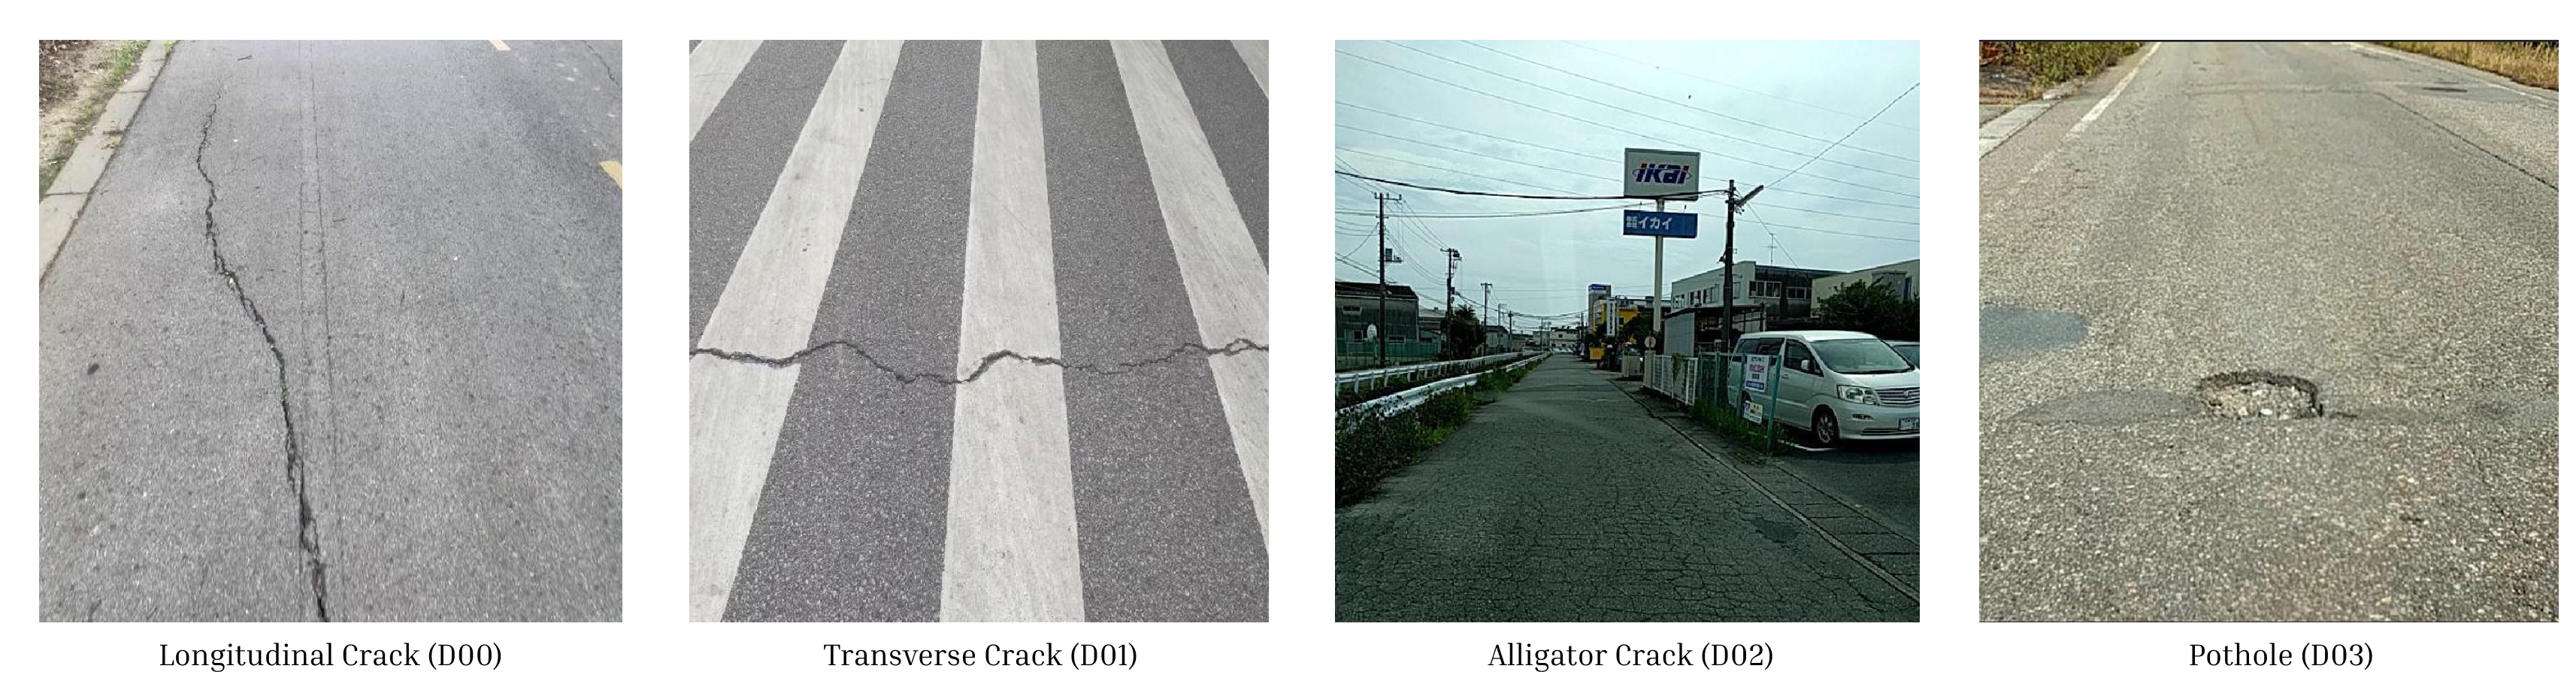
\includegraphics[width=\textwidth]{gambar/contoh_label_RDD.png}
  \caption{Contoh kerusakan jalan pada RDD2022 (D00, D10, D20, D40)}
  \label{fig:label_kerusakan_rdd}
\end{figure}

Meskipun RDD2022 telah memberikan kontribusi besar, dataset ini memiliki keterbatasan karena hanya berfokus pada kerusakan struktural utama dan mengabaikan elemen permukaan jalan lain yang memiliki kemiripan visual. Matouq dkk. menemukan bahwa mayoritas sistem deteksi kerusakan jalan sering kali gagal dan menghasilkan tingkat \textit{false positive} yang tinggi karena algoritma tidak mampu membedakan lubang jalan asli dengan elemen infrastruktur lain seperti penutup saluran air (\textit{manhole cover}) dan tambalan aspal (\textit{patching}) \cite{matouq2024ai}. Hal ini diperkuat oleh temuan Shi, yang mengonfirmasi bahwa penutup saluran air sangat sering dideteksi secara keliru sebagai lubang jalan, sehingga objek pengecoh tersebut mutlak perlu dianotasi secara terpisah saat melatih model \cite{Shi_2026}. Sejalan dengan tantangan tersebut, Kaya dan \c{C}odur memperkenalkan dataset N-RDD2024, sebuah perluasan dari RDD2022 yang menambahkan 10 kelas anomali dan cacat permukaan, termasuk kelas penutup saluran air (D70) dan jalan bertambal (D80) \cite{kaya2024nrdd2024}. Dalam konteks deteksi objek, kelas-kelas tambahan ini sangat krusial untuk difungsikan sebagai kelas pengecoh. Dengan melatih model untuk mengenali kelas D70 dan D80 secara eksplisit bersamaan dengan kelas kerusakan asli, model dapat belajar membedakan fitur visual yang mirip sehingga mampu menekan tingkat kesalahan deteksi di kondisi jalan nyata \cite{matouq2024ai, Shi_2026}.

Di sisi lain, pemanfaatan kelas yang beragam memunculkan tantangan baru berupa ketimpangan distribusi jumlah sampel latih (\textit{class imbalance}). Pada jalanan nyata, kerusakan berupa lubang jalan (\textit{pothole}) secara inheren memiliki frekuensi kemunculan yang jauh lebih sedikit dibandingkan dengan retakan memanjang atau melintang. Zeng dan Zhong membuktikan bahwa ketimpangan ini menyebabkan akurasi deteksi kelas lubang jalan (D40) pada model standar seperti YOLOv8 sering kali menjadi yang paling rendah, yang berujung pada terjadinya \textit{missed detection} (kegagalan deteksi) yang berulang \cite{Zeng2024}.  Oleh karena itu, arsitektur \textit{deep learning} yang digunakan memerlukan strategi khusus penanganan ketimpangan kelas pada tahap pelatihan, agar sensitivitas model terhadap kelas minoritas dapat tetap terjaga.

\section{\textit{You Only Look Once} (YOLO)}
Algoritma \textit{You Only Look Once} (YOLO) merupakan salah satu terobosan paling signifikan dalam bidang visi komputer yang diklasifikasikan sebagai detektor objek satu tahap (\textit{one-stage detector}) \cite{redmon2016you}. Berbeda dengan algoritma dua tahap (\textit{two-stage detector}) yang memerlukan proses pembuatan proposal wilayah (\textit{region proposal}) secara terpisah, YOLO mengubah rumusan masalah deteksi objek menjadi sebuah masalah regresi \textit{end-to-end} \cite{redmon2016you, Li2024}. Pendekatan ini memungkinkan jaringan saraf tiruan (\textit{neural network}) tunggal untuk memprediksi probabilitas kelas dan koordinat kotak pembatas (\textit{bounding box}) secara serentak dalam satu kali komputasi maju (\textit{single forward pass}), sehingga menghasilkan kecepatan inferensi yang sangat tinggi \cite{redmon2016you}.

Sejak pertama kali diperkenalkan oleh Joseph Redmon dkk. melalui iterasi YOLOv1, algoritma ini terus mengalami evolusi struktural yang pesat \cite{redmon2016you}. Redmon dkk. kemudian mengembangkan YOLOv2 (juga dikenal sebagai YOLO9000) dan YOLOv3, yang membawa peningkatan signifikan pada kemampuan deteksi objek melalui pengenalan jaringan residual, \textit{Spatial Pyramid Pooling} (SPP), dan \textit{Cross-Stage Partial Networks} (CSPNet) \cite{redmon2017yolo9000, redmon2018yolov3}. Evolusi arsitektur ini kemudian dilanjutkan oleh Bochkovskiy dkk. melalui peluncuran YOLOv4 pada tahun 2020, yang mengkonsolidasikan berbagai teknik optimasi mutakhir, termasuk augmentasi data \textit{Mosaic} dan modul atensi spasial, guna menawarkan detektor objek yang lebih optimal secara kecepatan maupun akurasi \cite{bochkovskiy2020yolov4}.

Iterasi baru dari keluarga algoritma ini, yaitu YOLOv8, dirilis oleh Ultralytics pada awal tahun 2023 dengan membawa pembaruan signifikan, termasuk penggunaan \textit{anchorless segmentation head} serta optimasi pada struktur jaringan \cite{Li2024}. Secara umum, arsitektur dasar jaringan YOLOv8 terbagi menjadi tiga komponen utama: \textit{Backbone} untuk ekstraksi fitur dari citra masukan, \textit{Neck} untuk melakukan fusi fitur multi-skala, dan \textit{Head} untuk menghasilkan prediksi akhir berupa lokasi, kelas, dan tingkat kepercayaan (\textit{confidence}) dari objek yang dideteksi \cite{Li2024, Zeng2024}.

% ==========================================
% GAMBAR 1: YOLOv8 STANDAR
% ==========================================
\begin{figure}[H]
  \centering
  % Gambar ini diambil dari Figure 3 pada Paper Li dkk. (2024)
  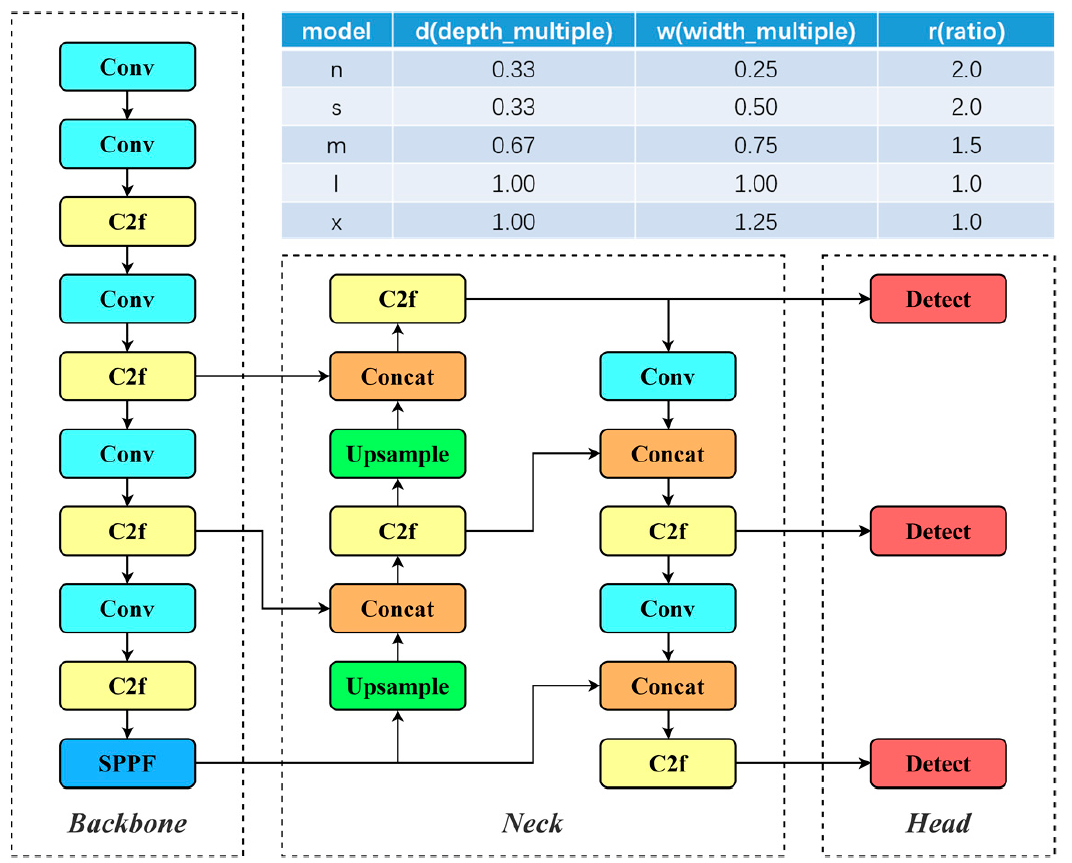
\includegraphics[width=0.85\textwidth]{gambar/arsitektur_yolov8_standar.png}
  \caption{Arsitektur Dasar Jaringan YOLOv8 (sumber: Li dkk., 2024 \cite{Li2024})}
  \label{fig:yolov8_standar}
\end{figure}

Algoritma YOLOv8 dirancang dengan tingkat fleksibilitas tinggi dan menyediakan lima varian berdasarkan skala kedalaman (\textit{depth}) dan lebar (\textit{width}) jaringan, yaitu YOLOv8n (nano), YOLOv8s (\textit{small}), YOLOv8m (\textit{medium}), YOLOv8l (\textit{large}), dan YOLOv8x (\textit{extra large}), sebagaimana yang diilustrasikan pada Gambar \ref{fig:yolov8_standar} \cite{Li2024}. Mengingat deteksi kerusakan jalan sering kali menuntut implementasi pada perangkat komputasi terbatas, varian yang paling ringan seperti YOLOv8n atau YOLOv8s menjadi kandidat \textit{baseline} yang paling ideal untuk meminimalkan beban komputasi.

\section{Modifikasi Arsitektur YOLO untuk Efisiensi}
Meskipun varian standar YOLOv8 telah memberikan performa yang baik, berbagai modifikasi struktural tingkat lanjut sering kali diperlukan untuk mengatasi tantangan spesifik pada citra jalan raya, seperti ukuran objek kerusakan yang sangat kecil (\textit{small objects}), latar belakang yang kompleks, serta keterbatasan memori perangkat.

Salah satu teknik modifikasi yang terbukti efektif adalah integrasi mekanisme atensi (\textit{attention mechanism}) ke dalam jaringan \cite{Wu2023, Li2024}. Mekanisme atensi, seperti \textit{Simple, Parameter-Free Attention Module} (SimAM) atau \textit{Convolutional Block Attention Module} (CBAM) \cite{woo2018cbam}, berfungsi untuk mengarahkan fokus model secara adaptif pada informasi visual yang krusial (seperti pola retakan tipis) sekaligus menekan gangguan (\textit{noise}) dari elemen visual latar belakang. Modul SimAM, misalnya, mampu menghitung bobot atensi tiga dimensi secara langsung dari fungsi energi neuron tanpa menambah beban parameter jaringan secara signifikan \cite{Li2024}.


% ==========================================
% GAMBAR 2: YOLOv8 MODIFIKASI
% ==========================================
\begin{figure}[H]
  \centering
  % Gambar ini diambil dari Figure 4 pada Paper Li dkk. (2024)
  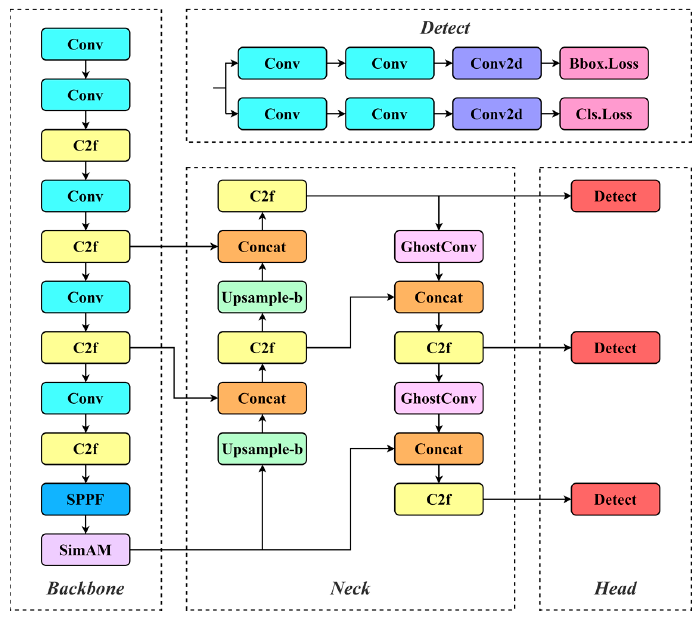
\includegraphics[width=0.85\textwidth]{gambar/arsitektur_yolov8_modifikasi.png}
  \caption{Contoh Modifikasi Arsitektur YOLOv8 yang Dioptimalkan untuk Efisiensi (sumber: Li dkk., 2024 \cite{Li2024})}
  \label{fig:yolov8_modifikasi}
\end{figure}

Selain mekanisme atensi, efisiensi model juga dapat ditingkatkan melalui modifikasi pada struktur konvolusi, sebagaimana diilustrasikan pada Gambar \ref{fig:yolov8_modifikasi}. Penggantian modul konvolusi standar pada bagian \textit{Neck} dengan \textit{Ghost Convolution} (\textit{GhostConv}) \cite{han2020ghostnet} mampu mereduksi redundansi fitur melalui operasi linear berbiaya rendah. Pendekatan ini secara drastis menurunkan jumlah parameter dan beban komputasi (GFLOPs) dengan tetap mempertahankan kemampuan ekstraksi fitur yang tangguh \cite{Zeng2024, Shi_2026}.

Di samping optimasi struktural, penanganan ketimpangan distribusi data (\textit{class imbalance}) mutlak diperlukan pada tahap pelatihan, terutama karena frekuensi kemunculan lubang jalan dan jalan bertambal jauh lebih sedikit dibandingkan dengan retakan memanjang dan buaya. Untuk mengatasi masalah ini secara stabil pada pelatihan presisi campuran (\textit{Automatic Mixed Precision} / AMP), pendekatan pembobotan kelas adaptif berbasis \textit{Effective Number of Samples} yang diperkenalkan oleh Cui dkk. \cite{cui2019class} diadopsi. Metode ini menghitung volume ruang fitur efektif yang dicakup oleh $n$ sampel menggunakan formulasi:
\begin{equation}
  E_n = \frac{1 - \beta^n}{1 - \beta}
\end{equation}
dengan $\beta \in [0, 1)$ sebagai hiperparameter yang merepresentasikan probabilitas tumpang tindih fitur. Bobot kerugian untuk setiap kelas $i$ kemudian dinormalisasi sebagai proporsi terbalik dari volume efektifnya:
\begin{equation}
  W_i = \frac{1 - \beta}{1 - \beta^{n_i}}
\end{equation}
Pendekatan ini mencegah ledakan bobot numerik ekstrem yang kerap terjadi pada skema pembobotan frekuensi terbalik mentah (\textit{inverse class frequency}), sehingga menjaga kestabilan konvergensi gradien tanpa mengabaikan penalti pada kelas minoritas \cite{cui2019class}. Penggabungan teknik atensi, konvolusi ringan, dan pembobotan kerugian efektif ini menjadi landasan kokoh bagi rancangan model deteksi yang tangguh dan seimbang.


\section{\textit{Domain Shift} dan Evaluasi \textit{Zero-Shot}}
Pengembangan model deteksi kerusakan jalan secara global sering dihadapkan pada masalah \textit{domain shift}, yaitu fenomena penurunan performa drastis ketika model yang dilatih pada dataset suatu wilayah diuji di wilayah lain \cite{Arya2024846}. Tantangan ini diyakini akan menjadi semakin kompleks ketika sistem deteksi diimplementasikan di Indonesia. Penelitian Hugo dkk. menunjukkan bahwa meskipun model telah dilatih secara spesifik menggunakan dataset jalanan lokal Indonesia, performa deteksinya masih tertahan pada tingkat moderat (F1-Score 59,7\%) \cite{hugo2025efficientdet}. Keterbatasan tersebut utamanya dipicu oleh tingginya kompleksitas fitur visual jalanan lokal serta kesulitan model dalam melakukan generalisasi pada data baru (\textit{unseen data}) \cite{hugo2025efficientdet}. Berdasarkan fakta tersebut, penerapan model yang dilatih secara eksklusif menggunakan dataset global, tanpa adanya representasi infrastruktur Indonesia, berpotensi kuat mengalami degradasi akurasi akibat fenomena \textit{domain shift}.


Untuk mengukur ketangguhan model secara objektif dalam menghadapi masalah tersebut, diterapkan skenario pengujian \textit{zero-shot}, yaitu mengevaluasi model yang dilatih pada data global secara langsung pada data primer jalan lokal tanpa melakukan pembelajaran ulang (\textit{fine-tuning}). Pengujian \textit{zero-shot} ini sangat relevan untuk diimplementasikan karena proses pengumpulan dan penganotasian ulang data kerusakan jalan secara spesifik untuk kebutuhan \textit{fine-tuning} membutuhkan waktu yang lama dan sangat menguras tenaga (\textit{time-consuming and labor-intensive}) \cite{matouq2024ai}. Oleh karena itu, evaluasi \textit{zero-shot} menjadi tolok ukur yang paling efisien untuk mengukur kemampuan generalisasi murni dari arsitektur \textit{deep learning} sebelum diterapkan secara nyata pada sistem pemantauan di Indonesia.

\section{Penelitian Terkait}
Penelitian mengenai deteksi kerusakan jalan berbasis \textit{deep learning} telah banyak dilakukan. Beberapa penelitian terdahulu telah mengusulkan berbagai modifikasi arsitektur YOLO maupun penggunaan dataset yang beragam. Meskipun demikian, sebagian besar model masih memiliki keterbatasan ketika dihadapkan pada masalah \textit{domain shift} dan tingginya tingkat \textit{false positive} akibat elemen pengecoh di jalan raya. Rincian perbandingan antara penelitian terdahulu (\textit{state-of-the-art}) dengan rencana penelitian ini dapat dilihat pada Tabel \ref{tab:penelitian_terkait}.

\small
\renewcommand{\arraystretch}{1.3}
\begin{longtable}{>{\raggedright}p{1.4cm}>{\raggedright}p{3.3cm}>{\raggedright\arraybackslash}p{7.8cm}}
  \caption{Kekurangan dan Kelebihan Penelitian Deteksi Kerusakan Jalan}\label{tab:penelitian_terkait}                                                                                                                                                                                                                                                                                                                                                                                                                             \\
  \hline
  \textbf{Sumber}             & \textbf{Metode \& Dataset}                                                                                                  & \textbf{Kelebihan \& Kekurangan}                                                                                                                                                                                                                                                                                                                                    \\
  \hline
  \endfirsthead
  \hline
  \textbf{Sumber}             & \textbf{Metode \& Dataset}                                                                                                  & \textbf{Kelebihan \& Kekurangan}                                                                                                                                                                                                                                                                                                                                    \\
  \hline
  \endhead
  \hline
  \endfoot
  \cite{Li2024}               & \textbf{Metode:} RDD-YOLO (YOLOv8 + SimAM + GhostConv) \newline \textbf{Dataset:} RDD2022                                   & \textbf{Kelebihan:} \newline $\bullet$ Mencapai akurasi mAP yang tinggi dengan beban komputasi yang lebih efisien dibandingkan YOLOv8 standar. \newline \textbf{Kekurangan:} \newline $\bullet$ Belum menguji efek \textit{domain shift} pada jalan di luar 6 negara dataset latih. \newline $\bullet$ Dataset tidak memuat anotasi kelas pengecoh secara spesifik. \\
  \hline
  \cite{Zeng2024}             & \textbf{Metode:} YOLOv8-PD (YOLOv8n + GhostNet) \newline \textbf{Dataset:} RDD2022                                          & \textbf{Kelebihan:} \newline $\bullet$ Arsitektur sangat ringan, berhasil menekan jumlah parameter komputasi hingga menjadi 2,3 juta parameter. \newline \textbf{Kekurangan:} \newline $\bullet$ Akurasi pada deteksi lubang jalan (D40) anjlok hingga 53,1\% dan sering gagal mendeteksi lubang kecil akibat ketimpangan kelas.                                    \\
  \hline
  \cite{matouq2024ai}         & \textbf{Metode:} YOLOv8 Instance Segmentation \newline \textbf{Dataset:} Data Custom Ohio                                   & \textbf{Kelebihan:} \newline $\bullet$ Membuktikan bahwa melatih kelas penutup saluran air dan tambalan jalan secara bersamaan terbukti menekan \textit{false positive}. \newline \textbf{Kekurangan:} \newline $\bullet$ Pengumpulan dan anotasi data mandiri memakan waktu dan membutuhkan komputasi yang sangat besar.                                           \\
  \hline
  \cite{hugo2025efficientdet} & \textbf{Metode:} EfficientDet-D0 \newline \textbf{Dataset:} Citra Jalan Indonesia                                           & \textbf{Kelebihan:} \newline $\bullet$ Menggunakan data jalan raya primer (lokal Indonesia) untuk evaluasi dan menggunakan fungsi \textit{loss} gabungan. \newline \textbf{Kekurangan:} \newline $\bullet$ Performa akurasi tertahan pada tingkat moderat (F1-Score 59,7\%) karena kesulitan model melakukan generalisasi fitur lokal.                              \\
  \hline
  \cite{Shi_2026}             & \textbf{Metode:} YOLO-LWD (GhostConv + ECA) \newline \textbf{Dataset:} Aug-RDD                                              & \textbf{Kelebihan:} \newline $\bullet$ Model sangat efisien secara komputasi dan menganotasi penutup saluran (\textit{manhole cover}) secara terpisah. \newline \textbf{Kekurangan:} \newline $\bullet$ Hanya divalidasi pada \textit{single domain} (jalan lokal Tiongkok), belum dievaluasi kemampuannya di negara lain.                                          \\
  \hline
  \textbf{Usulan}             & \textbf{Metode:} Evaluasi Komparatif YOLO \textit{lightweight} \newline \textbf{Dataset:} N-RDD2024 \& Jalan Raya Indonesia & \textbf{Kelebihan Rencana Penelitian:} \newline $\bullet$ Menggabungkan dataset global N-RDD2024 (dengan anotasi kelas pengecoh eksplisit) dan mengujinya secara \textit{zero-shot} langsung pada jalan Indonesia.                                                                                                                                                  \\
  \hline
\end{longtable}

Berdasarkan Tabel \ref{tab:penelitian_terkait}, terlihat bahwa sebagian besar model yang berkinerja tinggi dikembangkan menggunakan dataset global (seperti RDD2022) yang tidak mencakup kelas pengecoh secara eksplisit \cite{Li2024, Zeng2024}. Di sisi lain, penelitian yang telah menyoroti pentingnya kelas pengecoh seperti penutup saluran air dan tambalan aspal masih dievaluasi pada lingkungan yang terbatas (\textit{single domain}) \cite{matouq2024ai, Shi_2026}. Sementara itu, implementasi model deteksi secara langsung di Indonesia masih menunjukkan performa yang tertahan akibat kompleksitas fitur jalanan lokal \cite{hugo2025efficientdet}. Oleh karena itu, penelitian Tugas Akhir ini diusulkan untuk mengisi kesenjangan (\textit{research gap}) tersebut secara sistematis dengan melakukan evaluasi komparatif arsitektur YOLO \textit{lightweight} menggunakan dataset N-RDD2024, serta mengukur ketangguhan generalisasinya secara \textit{zero-shot} di domain jalan raya Indonesia.

%
\chapter{Metodologi dan Desain Sistem}

\section{Eksplorasi Data}
Eksplorasi data (\textit{Exploratory Data Analysis} / EDA) pada penelitian ini dilakukan untuk memahami karakteristik, distribusi, dan kualitas visual dari citra kerusakan jalan. Melalui analisis statistik dan visualisasi, EDA berperan penting dalam mengidentifikasi ketidakseimbangan kelas (\textit{class imbalance}) dan variasi ukuran objek untuk menentukan strategi pra-pemrosesan data yang tepat.

\subsection{Akuisisi Dataset}
Penelitian ini menggunakan dua jenis dataset yang diperoleh melalui metode akuisisi yang berbeda untuk memenuhi skenario pelatihan dan pengujian \textit{zero-shot}:
\begin{enumerate}
	\item \textbf{Data Sekunder (Dataset Pelatihan):} Dataset global \textcolor{blue}{\href{https://data.mendeley.com/datasets/27c8pwsd6v/3}{N-RDD2024}} yang merupakan perluasan dari RDD2022. Dari dataset ini, diekstraksi subset spesifik dari negara Asia (India, China, dan Jepang) dengan total 10.395 citra. Data ini sudah memiliki anotasi \textit{bounding box} untuk kelas kerusakan utama (D00, D10, D20, D40) serta kelas pengecoh (D70 untuk penutup saluran air dan D80 untuk tambalan jalan).
	\item \textbf{Data Primer (Dataset Pengujian \textit{Zero-Shot}):} Data citra jalan raya primer diakuisisi secara mandiri di wilayah Bandung. Pengambilan data difokuskan pada rute jalan raya dan jalan besar beraspal untuk merepresentasikan karakteristik infrastruktur lalu lintas utama di Indonesia. Target kuantitas data yang akan diekstraksi dan dianotasi adalah minimal 500 citra berlabel. Akuisisi dilakukan menggunakan kamera perekaman 1080p pada 30 fps dengan sudut pandang pengendara kendaraan roda dua pada kondisi siang hari. Frame diekstraksi dengan interval tertentu, misalnya setiap 1–2 detik atau berdasarkan perubahan \textit{scene}, untuk mengurangi redundansi visual antar citra. Karena data ini bersifat mentah, dilakukan pelabelan secara manual menggunakan perangkat lunak \textit{Computer Vision Annotation Tool} (CVAT) / Roboflow dengan format anotasi standar YOLO. Kualitas anotasi divalidasi secara manual untuk memastikan konsistensi label. Standar penarikan kotak pembatas (\textit{bounding box}) untuk seluruh kelas mengacu pada panduan contoh visual dari dataset N-RDD2024 beserta literatur basisnya, yakni RDD2022 \cite{Arya2024846}.

\end{enumerate}

\subsection{Visualisasi Data}
Tahap eksplorasi dan visualisasi data pada penelitian ini difokuskan pada subset data latih (\textit{training set}) N-RDD2024 dari tiga negara Asia: Jepang, Tiongkok, dan India. Mengingat dataset N-RDD2024 awalnya dikembangkan untuk keperluan kompetisi dengan label \textit{ground truth} pada data uji (\textit{test set}) yang dirahasiakan, maka seluruh proses eksplorasi ini hanya menggunakan data latih publik.

Dari total 10.395 citra awal, dilakukan proses penyaringan (\textit{filtering}) untuk mengekstraksi citra yang hanya memuat setidaknya satu dari enam kelas target penelitian (retakan memanjang, retakan melintang, retakan buaya, lubang jalan, penutup saluran, dan jalan bertambal). Proses penyaringan ini menghasilkan 9.670 citra siap pakai yang secara asli telah tersedia dalam format resolusi $640\times640$ piksel. Proporsi distribusi citra berdasarkan negara ditunjukkan pada Gambar \ref{fig:distribusi_negara}.

% ==========================================
% GAMBAR: DISTRIBUSI CITRA PER NEGARA
% ==========================================
\begin{figure}[H]
	\centering
	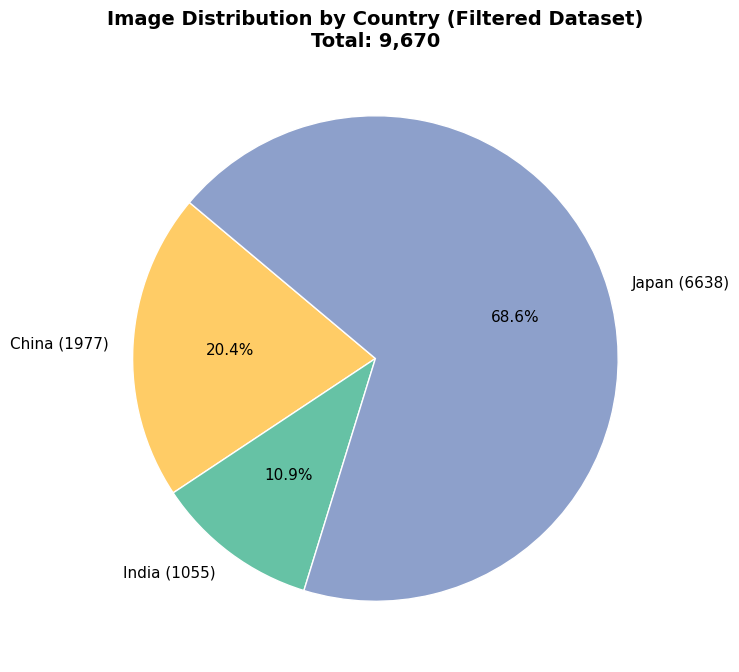
\includegraphics[width=0.7\textwidth]{gambar/distribusi_gambar.png} % Sesuaikan nama file
	\caption{Distribusi Citra N-RDD2024 Berdasarkan Negara}
	\label{fig:distribusi_negara}
\end{figure}

Berdasarkan Gambar \ref{fig:distribusi_negara}, terlihat bahwa dataset didominasi oleh citra dari Jepang sebanyak 6.638 citra (68,6\%), disusul oleh Tiongkok dengan 1.977 citra (20,4\%), dan India dengan 1.055 citra (10,9\%). Keragaman asal citra ini memunculkan variasi visual yang tinggi pada karakteristik jalan, sebagaimana divisualisasikan pada contoh citra anotasi kelas dan contoh perwakilan tiap negara di Gambar \ref{fig:contoh_kelas} dan Gambar \ref{fig:contoh_negara}.

% ==========================================
% GAMBAR: CONTOH KELAS
% ==========================================
\begin{figure}[H]
	\centering
	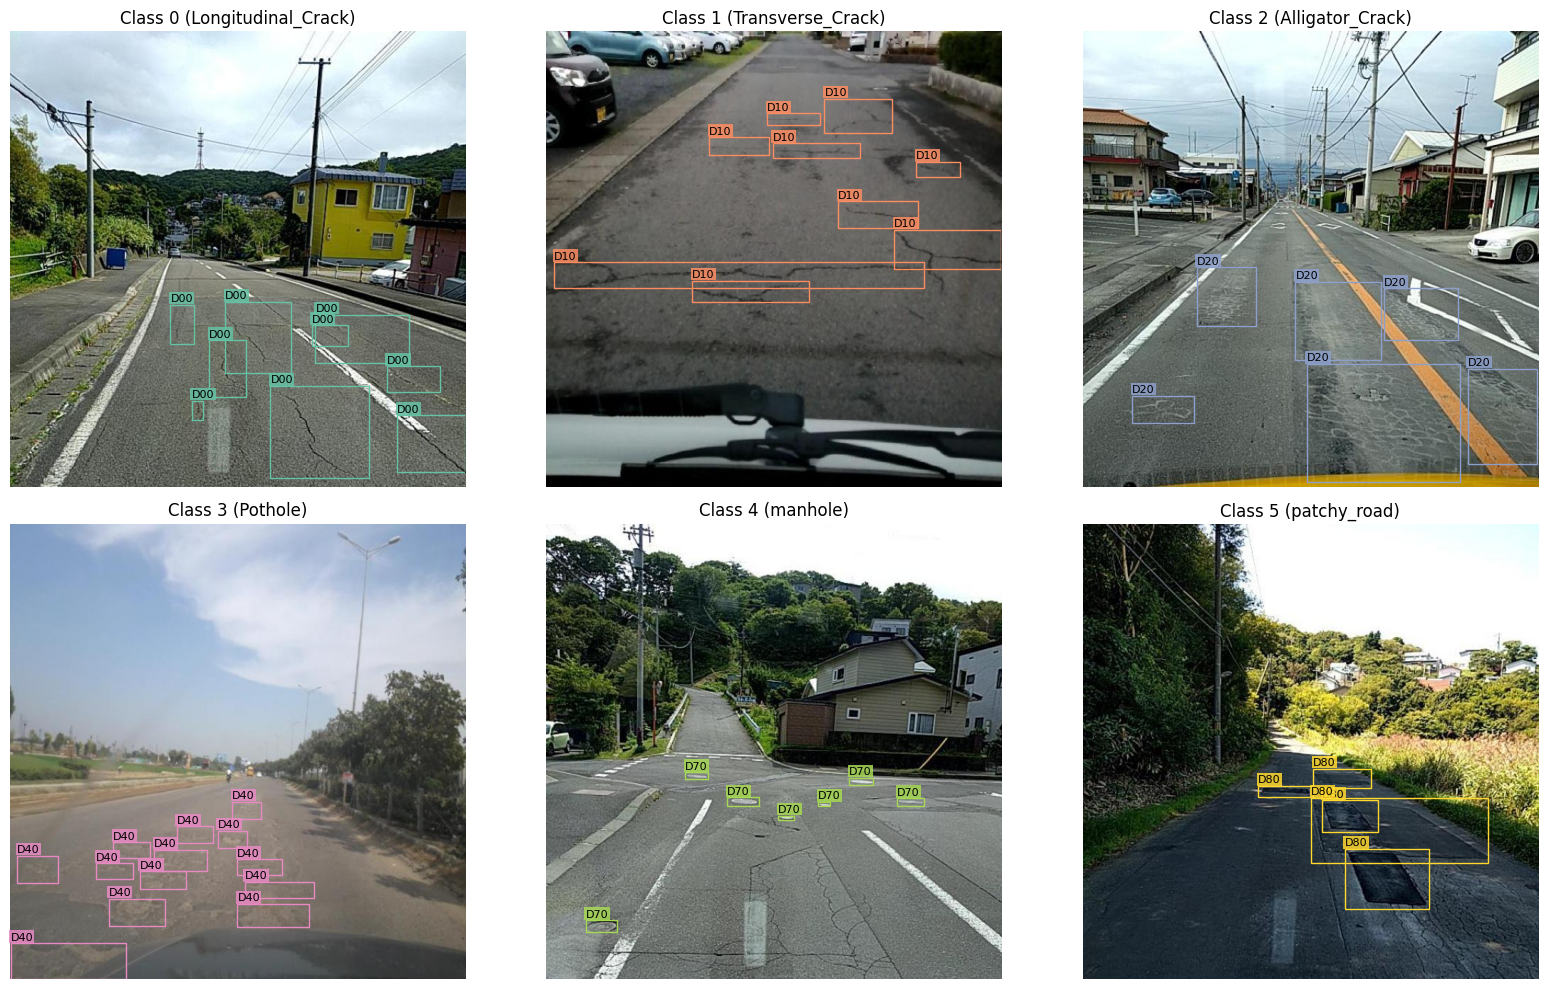
\includegraphics[width=0.9\textwidth]{gambar/object_sample.png} % Sesuaikan nama file
	\caption{Contoh Visualisasi \textit{Bounding Box} untuk Enam Kelas Target}
	\label{fig:contoh_kelas}
\end{figure}

% ==========================================
% GAMBAR: CONTOH NEGARA
% ==========================================
\begin{figure}[H]
	\centering
	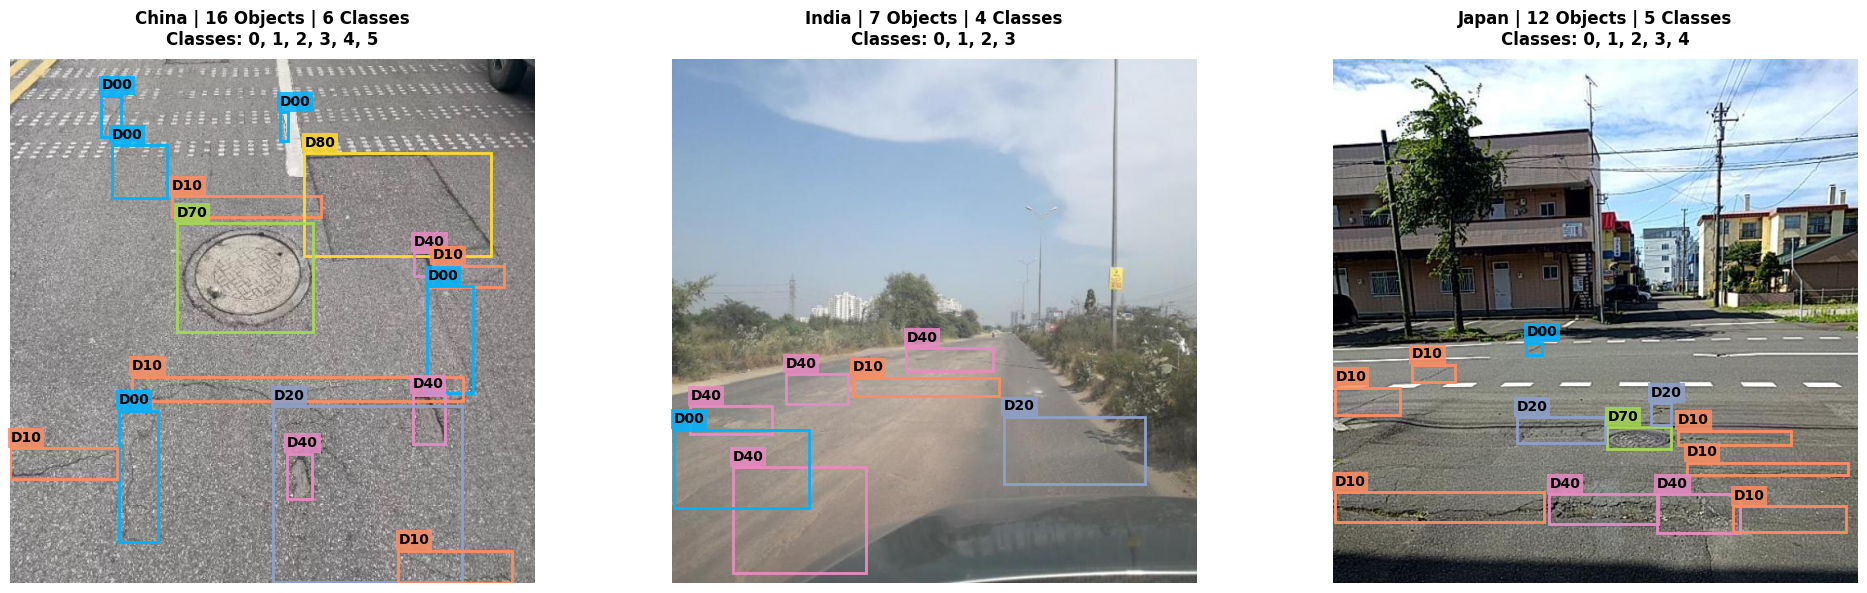
\includegraphics[width=0.9\textwidth]{gambar/object_per_country.png} % Sesuaikan nama file
	\caption{Contoh Perbedaan Karakteristik Citra Jalan di tiap Negara}
	\label{fig:contoh_negara}
\end{figure}

Selain asal negara, tantangan utama dari dataset ini terletak pada ketimpangan distribusi jumlah objek antar kelas (\textit{class imbalance}). Analisis terhadap total 24.290 objek berlabel menunjukkan bahwa kelas retakan struktural sangat mendominasi dibandingkan kelas anomali permukaan lainnya.

% ==========================================
% GAMBAR: DISTRIBUSI KELAS GLOBAL
% ==========================================
\begin{figure}[H]
	\centering
	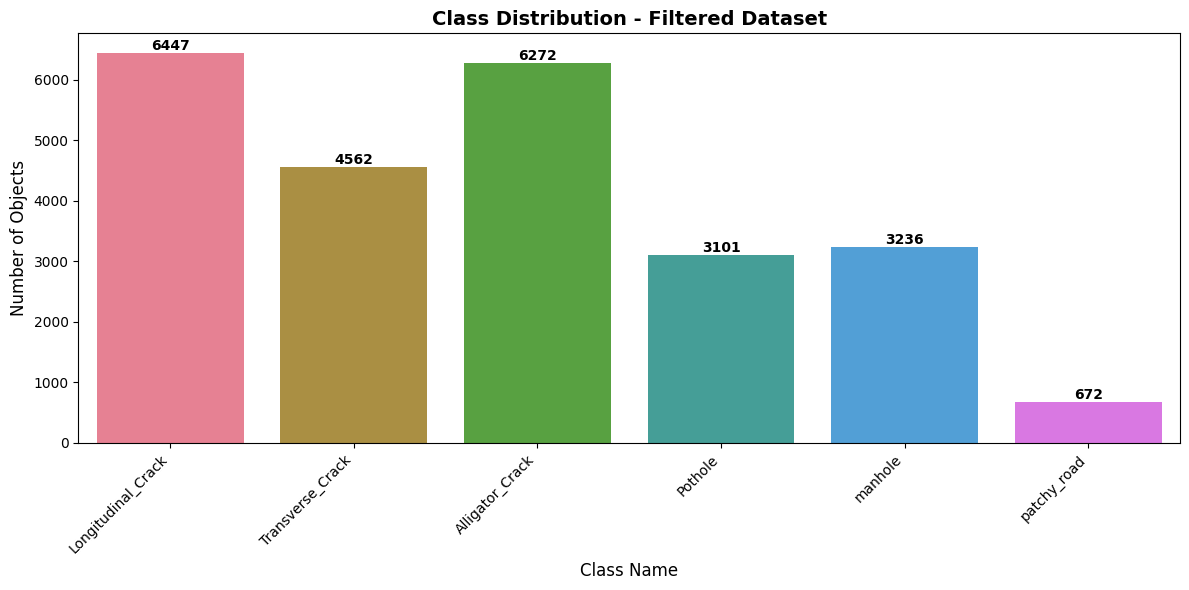
\includegraphics[width=0.85\textwidth]{gambar/distribusi_kelas.png} % Sesuaikan nama file
	\caption{Distribusi Jumlah Objek Berdasarkan Kelas pada Dataset Tersaring}
	\label{fig:distribusi_kelas_global}
\end{figure}

Merujuk pada Gambar \ref{fig:distribusi_kelas_global}, retakan memanjang dan retakan buaya secara berurutan mencatatkan jumlah terbanyak, yaitu 6.447 dan 6.272 objek. Sebaliknya, kelas jalan bertambal (\textit{patchy road}) sangat langka dengan hanya 672 objek. Kelas lubang jalan (\textit{pothole}) dan penutup saluran (\textit{manhole}) juga berada pada kategori minoritas (masing-masing 3.101 dan 3.236 objek). Ketimpangan ini semakin terlihat kompleks ketika dibedah berdasarkan sebaran tiap negara, seperti yang disajikan pada Gambar \ref{fig:distribusi_objek_negara}.

% ==========================================
% GAMBAR: DISTRIBUSI KELAS PER NEGARA
% ==========================================
\begin{figure}[H]
	\centering
	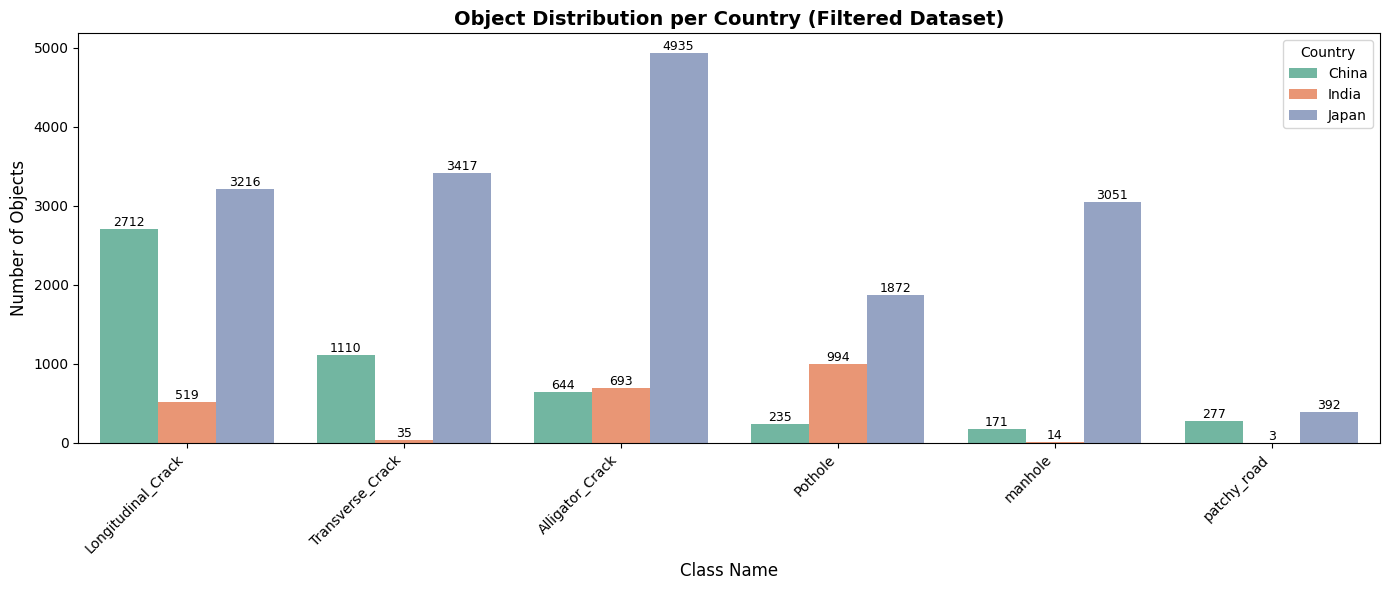
\includegraphics[width=0.9\textwidth]{gambar/distribusi_kelas_country.png} % Sesuaikan nama file
	\caption{Sebaran Jumlah Objek Spesifik per Kelas di Masing-masing Negara}
	\label{fig:distribusi_objek_negara}
\end{figure}

Data dari Gambar \ref{fig:distribusi_objek_negara} menyoroti anomali distribusi lokal. Sebagai contoh, sebagian besar objek \textit{manhole} (3.051 dari 3.236 objek) secara eksklusif bersumber dari Jepang, sementara objek lubang jalan (\textit{pothole}) memiliki proporsi kemunculan yang cukup tinggi di India (994 objek dari total 1.055 citra India) dibandingkan negara lainnya. Fakta empiris terkait ketimpangan kelas yang ekstrem ini menjustifikasi perlunya penerapan modifikasi struktural dan fungsi kerugian adaptif, seperti \textit{Focal Loss}, guna mencegah model bias terhadap kelas mayoritas (retakan) dan mengabaikan objek minoritas (lubang dan pengecoh).

Analisis komprehensif terhadap 24.290 kotak pembatas (\textit{bounding box}) pada dataset tersaring dilakukan untuk melihat proporsi luas objek relatif terhadap luas total citra. Hasil dari analisis metrik tersebut divisualisasikan melalui histogram pada Gambar \ref{fig:distribusi_luas_bbox}.

% ==========================================
% GAMBAR: DISTRIBUSI LUAS BBOX
% ==========================================
\begin{figure}[H]
	\centering
	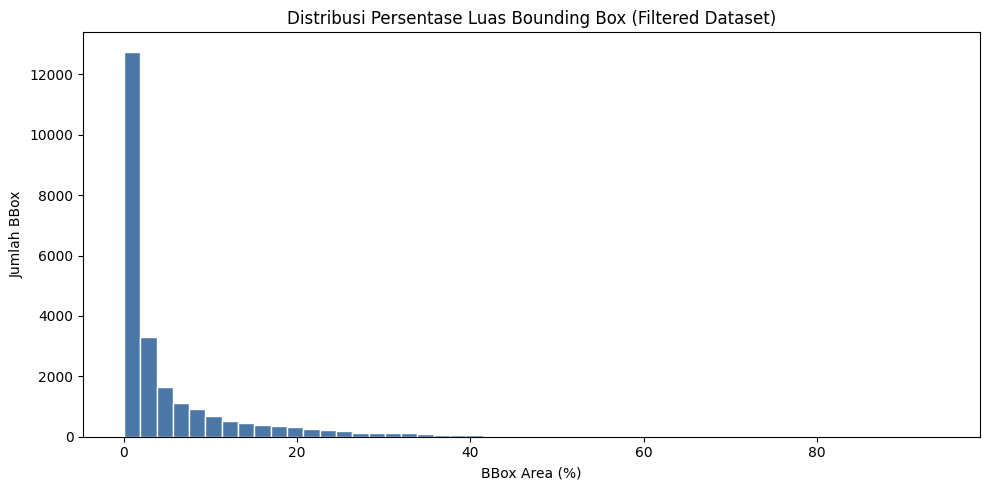
\includegraphics[width=0.9\textwidth]{gambar/distribusi_luas.png} % Sesuaikan nama file
	\caption{Distribusi Persentase Luas \textit{Bounding Box} Terhadap Luas Citra}
	\label{fig:distribusi_luas_bbox}
\end{figure}

Berdasarkan Gambar \ref{fig:distribusi_luas_bbox}, distribusi persentase luas \textit{bounding box} menunjukkan kecondongan positif yang sangat ekstrem (\textit{highly right-skewed}). Nilai median tercatat pada angka 1,69\%, yang mengindikasikan bahwa separuh dari total keseluruhan objek target pada dataset berukuran kurang dari 1,7\% dari total keseluruhan area piksel gambar. Lebih lanjut, metrik persentil ke-90 (P90) yang hanya menyentuh angka 17,19\% menegaskan bahwa keberadaan objek kerusakan berukuran besar sangat jarang ditemukan di lapangan.

Banyaknya objek berukuran sangat kecil dalam dataset ini menjadi tantangan visual tersendiri. Ukuran target yang minim, ditambah dengan tekstur latar belakang jalan raya yang kompleks, membuat anomali tersebut secara alami lebih sulit untuk dikenali secara akurat dalam proses deteksi.

\section{Alur Penelitian}
Penelitian ini dilaksanakan berdasarkan alur penelitian yang dirancang secara terstruktur dan sistematis. Rangkaian tahapan dari proses akuisisi data hingga penarikan kesimpulan divisualisasikan pada diagram alir (\textit{flowchart}) di Gambar \ref{fig:alur_penelitian}.

% ==========================================
% TEMPAT GAMBAR FLOWCHART
% ==========================================
\begin{figure}[H]
	\centering
	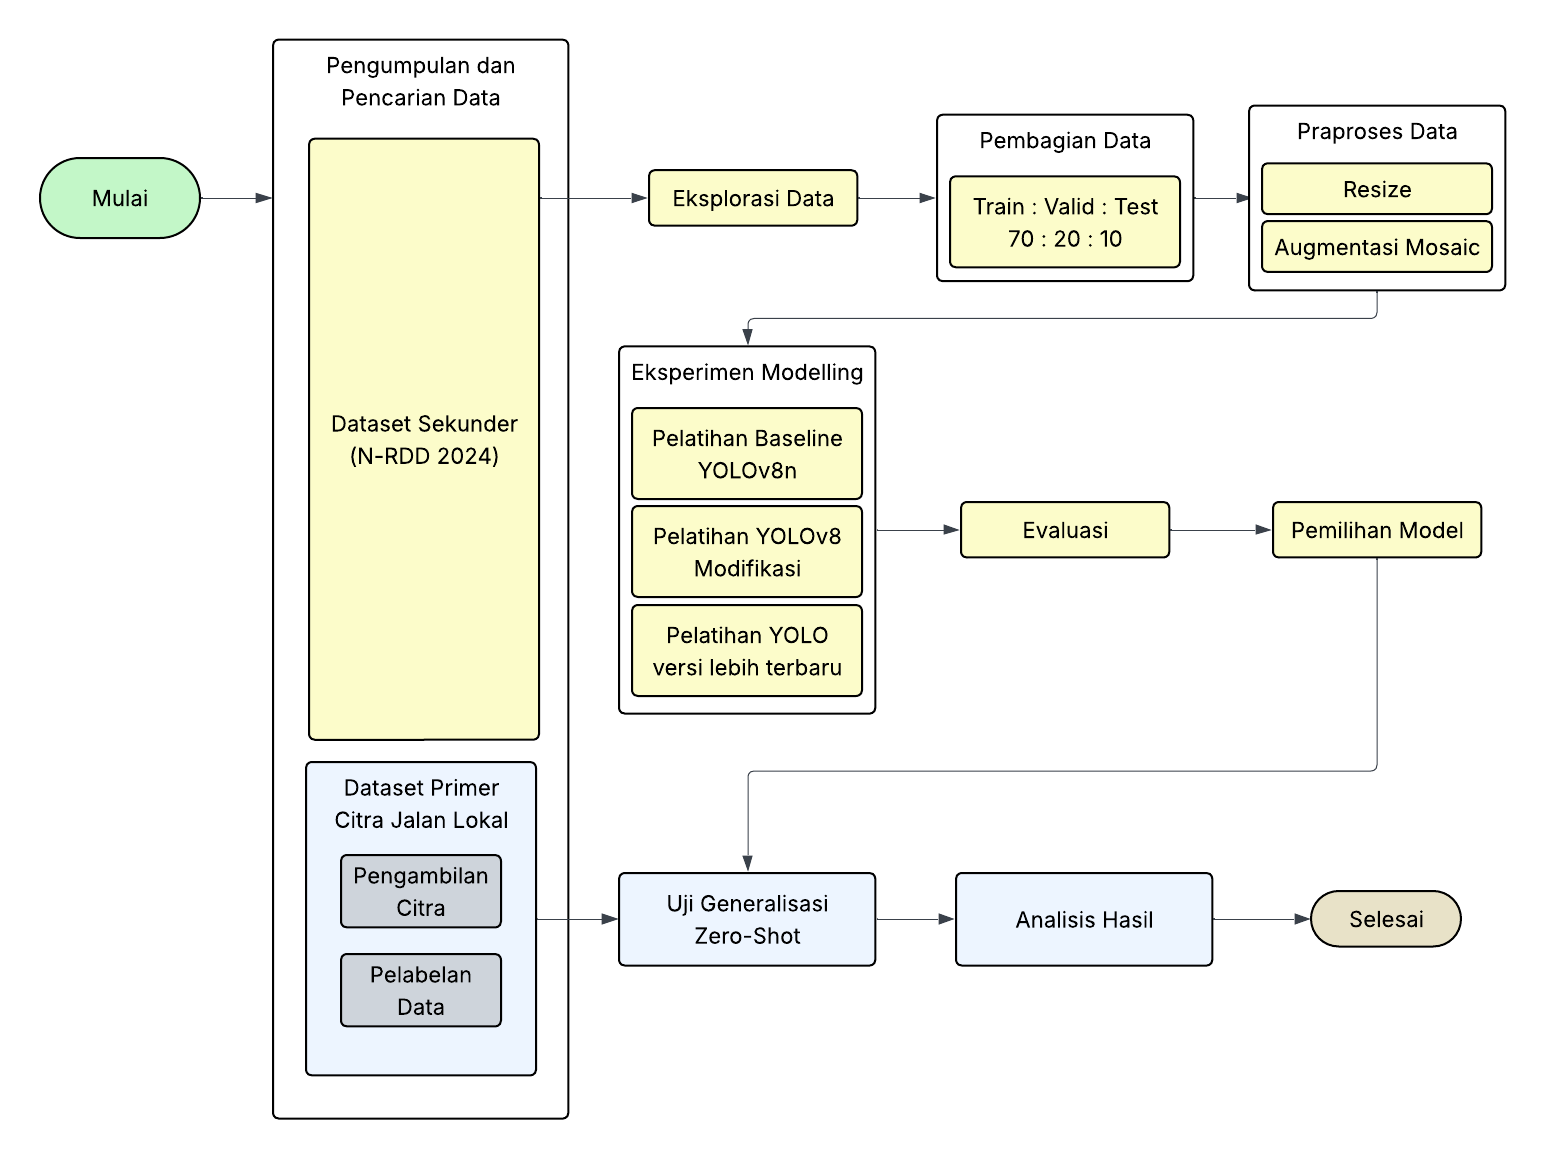
\includegraphics[width=1\textwidth]{gambar/flowchart_penelitian.png}
	\caption{Flowchart Alur Penelitian}
	\label{fig:alur_penelitian}
\end{figure}

Penelitian dimulai dengan pengumpulan data yang terbagi menjadi dua domain utama. Pertama, akuisisi data sekunder menggunakan dataset global \textcolor{blue}{\href{https://data.mendeley.com/datasets/27c8pwsd6v/3}{N-RDD2024}} yang memiliki label kelas kerusakan dan kelas pengecoh secara komprehensif \cite{kaya2024nrdd2024}. Kedua, akuisisi data primer berupa citra jalan raya lokal di  Bandung yang diambil secara mandiri. Karena data primer yang terkumpul masih bersifat mentah, maka dilakukan proses pelabelan secara manual dengan memberikan kotak pembatas (\textit{bounding box}) menggunakan format anotasi standar YOLO agar sesuai dengan kebutuhan inferensi model nantinya.

Setelah data terkumpul, tahap selanjutnya adalah Eksplorasi Data (\textit{Exploratory Data Analysis} / EDA) untuk menganalisis distribusi kelas, ketimpangan data, serta variasi ukuran anomali permukaan jalan. Pemahaman terhadap karakteristik data ini menjadi landasan untuk membagi dataset sekunder (\textit{data splitting}) menjadi himpunan data latih (\textit{train}), data validasi (\textit{validation}), dan data uji (\textit{test}) dengan proporsi 70:20:10.

Himpunan data tersebut kemudian melalui tahap pra-pemrosesan (\textit{preprocessing}). Tahap ini difokuskan pada penyesuaian resolusi citra (\textit{resizing}) menjadi $640 \times 640$ piksel agar sesuai dengan standar ukuran arsitektur masukan (\textit{input size}) keluarga algoritma YOLO \cite{Zeng2024}. Selanjutnya, dilakukan normalisasi nilai piksel serta penerapan teknik augmentasi data seperti \textit{Mosaic}. Augmentasi \textit{Mosaic} bekerja dengan cara menggabungkan empat citra berbeda menjadi satu masukan tunggal, yang secara efektif memperkaya variasi fitur spasial dan melatih model untuk lebih kebal terhadap latar belakang yang kompleks serta variasi skala objek \cite{Zeng2024}.

Tahap pemodelan merancang tiga skenario eksperimen komparatif. Skenario pertama adalah pelatihan model \textit{baseline} menggunakan varian YOLOv8n. Skenario kedua merupakan pelatihan menggunakan arsitektur YOLO yang dimodifikasi (mengikuti penyesuaian arsitektur dari literatur referensi yang relevan dengan dataset). Skenario ketiga menggunakan iterasi algoritma YOLO versi yang lebih baru (seperti YOLOv12 \cite{tian2026yolov12} dan YOLOv26 \cite{sapkota2025yolo26}). Skenario ketiga ini sangat krusial untuk mengevaluasi dan membandingkan apakah peningkatan arsitektur bawaan (\textit{native}) dari versi mutakhir mampu memberikan performa yang lebih tangguh dibandingkan dengan rancangan modifikasi struktural pada iterasi YOLO \textit{baseline}.

Ketiga skenario model tersebut kemudian dievaluasi menggunakan metrik performa deteksi dan metrik efisiensi komputasi untuk menentukan arsitektur dengan keseimbangan kinerja terbaik. Sebagai puncak dari pengujian, model terbaik yang diperoleh dari pelatihan data sekunder akan langsung diuji kemampuannya dalam melakukan generalisasi (\textit{zero-shot inference}) menggunakan dataset primer jalan raya lokal. Uji inferensi ini dilakukan tanpa melatih ulang (\textit{fine-tuning}) model pada data primer, guna mengukur secara objektif ketangguhan arsitektur dalam menghadapi fenomena \textit{domain shift}. Penelitian diakhiri dengan analisis hasil komprehensif atas inferensi \textit{zero-shot} dan penarikan kesimpulan.


\section{Rancangan Arsitektur Model}
Algoritma deteksi objek berbasis keluarga YOLO beroperasi sebagai detektor satu tahap (\textit{one-stage detector}) yang memproses citra secara serentak (\textit{end-to-end}). Pada tahap awal, citra masukan dibagi ke dalam kisi spasial (\textit{grid}) berukuran $S \times S$. Setiap sel pada kisi tersebut secara independen bertanggung jawab untuk memprediksi kotak pembatas (\textit{bounding box}) beserta probabilitas kelas dari objek yang pusat lokasinya jatuh di dalam area sel tersebut \cite{Li2024, Wang2025}. Alur kerja dan topologi dasar dari rancangan arsitektur ini divisualisasikan pada Gambar \ref{fig:arsitektur_yolo}.

% ==========================================
% GAMBAR: ILUSTRASI ARSITEKTUR YOLO
% ==========================================
\begin{figure}[H]
	\centering
	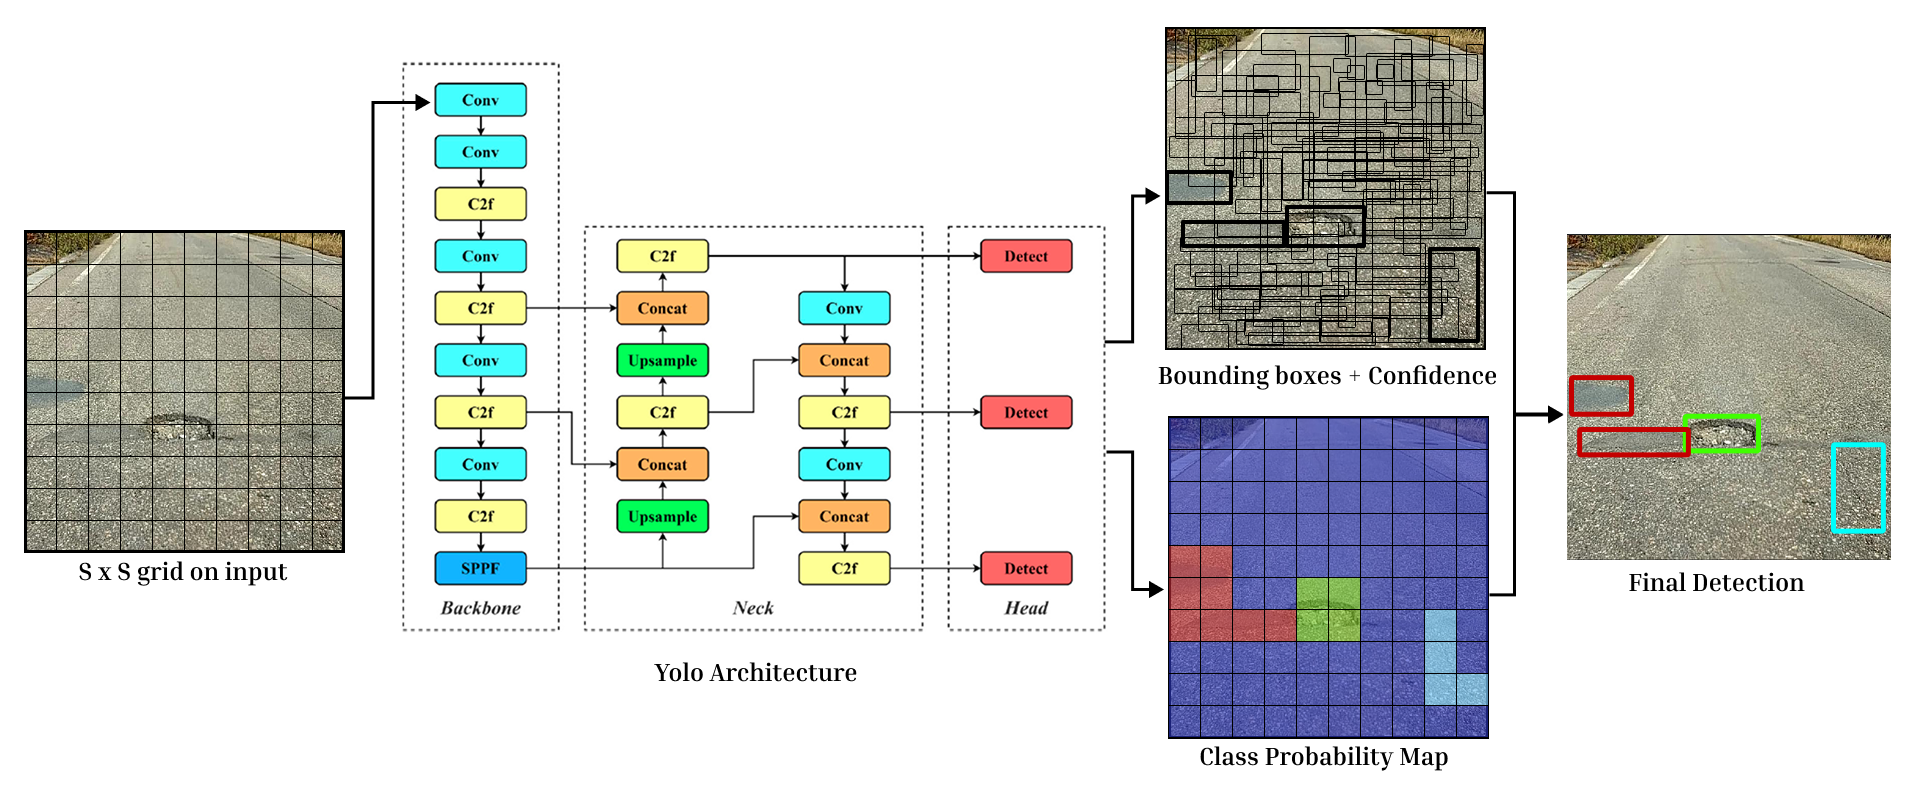
\includegraphics[width=0.9\textwidth]{gambar/rancangan_implementasi.png}
	\caption{Ilustrasi Alur Kerja dan Arsitektur Dasar Jaringan YOLO}
	\label{fig:arsitektur_yolo}
\end{figure}

Secara struktural, rancangan implementasi model jaringan YOLO pada penelitian ini bertumpu pada tiga komponen arsitektur utama, yaitu:
\begin{enumerate}
	\item \textbf{\textit{Backbone}:} Berfungsi sebagai pengekstraksi fitur utama dari citra masukan. Pada iterasi arsitektur mutakhir seperti YOLOv8, komponen ini memanfaatkan kombinasi modul konvolusi standar (Conv), modul C2f (\textit{Cross Stage Partial Bottleneck with 2 convolutions}) untuk memastikan aliran gradien yang kaya dan efisien selama propagasi balik, serta \textit{Spatial Pyramid Pooling - Fast} (SPPF) untuk mengekstrak fitur pada berbagai skala abstraksi spasial \cite{Li2024, Zeng2024}. Untuk meningkatkan sensitivitas terhadap objek berukuran kecil (seperti retakan halus), komponen \textit{backbone} ini sering kali menjadi target utama penyisipan mekanisme atensi, seperti modul SimAM \cite{Li2024} maupun SOM \cite{Wang2025}.

	\item \textbf{\textit{Neck}:} Bertugas melakukan fusi fitur multi-skala. Melalui hierarki operasi \textit{Upsample} dan penggabungan (\textit{Concatenation}), bagian ini memadukan peta fitur beresolusi tinggi (yang kaya akan detail spasial) dengan peta fitur beresolusi rendah (yang kaya akan informasi semantik global) \cite{Li2024, Shi_2026}. Fusi ini memungkinkan model untuk secara adaptif mengenali objek kerusakan jalan dalam rentang skala yang bervariasi. Pada implementasi model modifikasi (\textit{lightweight}), modul konvolusi standar pada \textit{Neck} umumnya digantikan oleh operasi linear hemat biaya seperti \textit{Ghost Convolution} guna mereduksi beban komputasi (GFLOPs) dan menekan redundansi parameter secara drastis \cite{Li2024, Zeng2024, Shi_2026}.

	\item \textbf{\textit{Head}:} Merupakan komponen akhir jaringan yang mengadopsi struktur \textit{decoupled head} untuk memisahkan tugas klasifikasi dan pelokalisasian secara independen. Bagian ini memproses fitur hasil fusi dari \textit{Neck} guna menghasilkan keluaran prediksi secara paralel, yaitu koordinat kotak pelingkup (\textit{bounding boxes}), tingkat metrik keyakinan (\textit{confidence score}), dan probabilitas kelas (\textit{class probability map}) \cite{Li2024, Shi_2026}. Prediksi mentah yang saling tumpang tindih kemudian disaring melalui algoritma \textit{Non-Maximum Suppression} (NMS) untuk menghasilkan keputusan deteksi akhir yang tunggal dan presisi.
\end{enumerate}

\section{Evaluasi Performa Model}
Evaluasi kinerja model pada penelitian ini dibagi menjadi dua aspek utama, yaitu evaluasi ketepatan deteksi (akurasi) dan evaluasi efisiensi komputasi model. Metrik-metrik ini krusial untuk mengukur keberhasilan model, terutama ketika diimplementasikan pada skenario \textit{real-time} dan perangkat dengan sumber daya terbatas \cite{Wu2023}.

\subsection{\textit{Confusion Matrix} (TP, FP, FN)}
Dalam tugas deteksi objek, landasan utama perhitungan metrik evaluasi bersumber dari \textit{Confusion Matrix} yang didefinisikan berdasarkan ambang batas \textit{Intersection over Union} (IoU). Matriks ini mengelompokkan hasil prediksi ke dalam tiga kondisi \cite{Li2024, Zeng2024}:
\begin{itemize}
	\item \textbf{\textit{True Positive} (TP):} Model berhasil memprediksi objek kerusakan jalan dengan benar, kelasnya sesuai dengan \textit{ground truth}, dan nilai IoU melampaui ambang batas yang ditentukan (misalnya IoU $>$ 0,5).
	\item \textbf{\textit{False Positive} (FP):} Model mendeteksi adanya objek kerusakan jalan di lokasi tertentu, padahal pada kondisi asli (\textit{ground truth}) tidak terdapat kerusakan (salah deteksi) atau kelas yang diprediksi keliru.
	\item \textbf{\textit{False Negative} (FN):} Terdapat kerusakan jalan pada kondisi nyata, namun model gagal mendeteksi atau melokalisasi kerusakan tersebut (\textit{missed detection}).
\end{itemize}

\subsection{\textit{Precision, Recall}, dan F1-\textit{Score}}
Berdasarkan nilai TP, FP, dan FN, kinerja klasifikasi model dapat diukur menggunakan tiga metrik turunan. \textit{Precision} mengukur tingkat ketepatan prediksi positif dari model, sedangkan \textit{Recall} (sensitivitas) mengukur kemampuan model dalam menemukan seluruh objek kerusakan yang sebenarnya ada di dalam citra \cite{Zeng2024, Li2024}.
\begin{equation}
	Precision = \frac{TP}{TP + FP}
\end{equation}
\begin{equation}
	Recall = \frac{TP}{TP + FN}
\end{equation}
Karena \textit{Precision} dan \textit{Recall} sering kali berbanding terbalik, digunakan metrik F1-\textit{Score} yang merupakan rata-rata harmonis dari keduanya. Metrik ini memberikan penilaian yang seimbang dan komprehensif terkait ketangguhan model \cite{Li2024}.
\begin{equation}
	F1\text{-}Score = 2 \times \frac{Precision \times Recall}{Precision + Recall}
\end{equation}

\subsection{\textit{Intersection over Union} (IoU) dan \textit{Mean Average Precision} (mAP)}
\textit{Intersection over Union} (IoU) mengukur seberapa akurat lokalisasi kotak pembatas (\textit{bounding box}) yang diprediksi oleh model dibandingkan dengan kotak pembatas asli (\textit{ground truth}) \cite{Li2024}.
\begin{equation}
	IoU = \frac{Area \ of \ Overlap}{Area \ of \ Union}
\end{equation}
Dari perhitungan presisi pada berbagai ambang batas \textit{Recall}, diperoleh nilai \textit{Average Precision} (AP). Rata-rata AP dari seluruh kelas objek kemudian dirumuskan menjadi \textit{Mean Average Precision} (mAP), yang merupakan metrik standar tertinggi dalam deteksi objek \cite{Wu2023, Li2024}:
\begin{equation}
	mAP = \frac{1}{N} \sum_{i=1}^{N} AP_i
\end{equation}
Dalam penelitian ini, selain menggunakan metrik mAP@0.5 (mAP pada IoU 50\%), digunakan pula metrik evaluasi multi-skala seperti mAP$_s$ (untuk objek berukuran sangat kecil $< 32\times32$ piksel), mAP$_m$ (skala menengah), dan mAP$_l$ (skala besar) untuk menganalisis sensitivitas model terhadap variasi ukuran retakan jalan yang ekstrem \cite{Wang2025}.

\subsection{Metrik Efisiensi Komputasi}
Untuk mengukur kelayakan model pada perangkat komputasi bergerak (\textit{mobile terminal devices}), digunakan tiga metrik evaluasi efisiensi \cite{Wu2023, Wang2025}:
\begin{itemize}
	\item \textbf{\textit{Parameters} (Params):} Total kuantitas bobot yang dapat dipelajari (\textit{learnable parameters}) dalam jaringan saraf. Metrik ini, biasanya dalam satuan \textit{Million} (M), mengukur kompleksitas spasial dan ukuran ruang penyimpanan model.
	\item \textbf{GFLOPs (\textit{Giga Floating-Point Operations Per Second}):} Kuantitas operasi komputasi yang dibutuhkan model dalam satu kali inferensi. Metrik ini secara langsung merepresentasikan beban komputasi jaringan.
	\item \textbf{FPS (\textit{Frames Per Second}):} Indikator langsung dari kecepatan inferensi model dalam memproses citra per detiknya, yang menentukan kelayakan sistem untuk skenario pengawasan \textit{real-time}.
\end{itemize}

\section{Skenario Penelitian}
Skenario pengujian merupakan inti eksperimental dari metodologi penelitian ini. Untuk menjawab ketiga rumusan masalah yang telah ditetapkan pada Bab 1 secara sistematis, skenario penelitian ini dipecah ke dalam tiga tahapan evaluasi utama:

\subsection{Skenario 1: Evaluasi Kinerja pada Domain Sumber dan Analisis Kelas Pengecoh}
Skenario pertama dirancang secara komparatif untuk melatih dan mengevaluasi konfigurasi arsitektur model menggunakan dataset sekunder N-RDD2024. Penelitian ini menguji YOLOv8n sebagai model \textit{baseline}, rancangan eksperimental model modifikasi yang dikonfigurasi dengan mengeksplorasi berbagai modul optimasi (seperti mekanisme atensi dan konvolusi ringan) yang diadaptasi dari arsitektur mutakhir seperti YOLO-RD \cite{Wang2025}, RDD-YOLO \cite{Li2024}, maupun YOLOv8-PD \cite{Zeng2024}, serta iterasi algoritma versi mutakhir berupa YOLOv12 \cite{tian2026yolov12} dan YOLOv26 \cite{sapkota2025yolo26}. Fokus utama pada tahap ini adalah mengukur tingkat akurasi (mAP) dari masing-masing arsitektur dalam mendeteksi kelas kerusakan jalan utama. Bersamaan dengan itu, evaluasi juga diarahkan untuk mengamati bagaimana model menangani ketimpangan data (\textit{class imbalance}) serta kemampuannya dalam membedakan kerusakan jalan asli dari kelas pengecoh berupa penutup saluran air (D70) dan tambalan aspal (D80). Kemampuan arsitektur dalam menghindari kebingungan visual terhadap objek pengecoh ini dibuktikan secara empiris melalui analisis maatriks kebingungan (\textit{Confusion Matrix}) guna melihat tingkat penekanan \textit{false positive}. Untuk memastikan model tidak bias terhadap kelas mayoritas selama proses pelatihan, strategi penanganan ketimpangan kelas melalui penerapan fungsi kerugian adaptif (\textit{Focal Loss}) atau pembobotan kelas bawaan dari kerangka kerja YOLO. Skenario ini akan menghasilkan capaian metrik mAP dan F1-\textit{Score} murni pada domain sumber yang menjadi \textit{benchmark} performa standar model.


\subsection{Skenario 2: Analisis Keseimbangan Kinerja (\textit{Trade-Off}) dan Kelayakan \textit{Real-Time}}
Skenario kedua berfokus pada analisis kelayakan penerapan model pada skenario \textit{real-time} dengan sumber daya komputasi terbatas. Pada tahap ini, metrik akurasi (mAP) dari model-model yang telah dilatih pada Skenario 1 akan dibandingkan dengan metrik efisiensi komputasinya, yang meliputi kecepatan inferensi (FPS), jumlah parameter (\textit{Params}), dan beban operasi (\textit{GFLOPs}). Seluruh pengujian efisiensi komputasi ini akan dievaluasi menggunakan perangkat keras NVIDIA RTX 4070 Ti 12GB sebagai basis tolok ukur (benchmark).Analisis keseimbangan kinerja (\textit{trade-off}) ini akan menentukan apakah modifikasi arsitektur \textit{lightweight} benar-benar mampu memberikan titik optimal terbaik antara menekan beban komputasi secara signifikan tanpa mengorbankan ketepatan deteksi. Dari skenario evaluasi komputasi ini, akan dipilih satu model terbaik untuk dilanjutkan ke tahap evaluasi akhir.

\subsection{Skenario 3: Uji Ketangguhan Lintas Domain (\textit{Zero-Shot Inference})}
Skenario ketiga bertujuan untuk mengukur secara kuantitatif tingkat kesenjangan domain (\textit{domain gap}) dari model terbaik yang telah terpilih. Model terbaik dari hasil analisis komputasi Skenario 2 akan diekstraksi bobotnya (\textit{weights}) dan diuji secara langsung (\textit{zero-shot}) menggunakan dataset primer jalan raya Bandung, tanpa memberikan model kesempatan untuk melakukan \textit{fine-tuning}. tahap evaluasi akhir ini akan membuktikan kemampuan generalisasi murni model dalam menghadapi data baru (\textit{unseen data}). Perbedaan selisih akurasi (\textit{accuracy drop}) antara kinerja di Skenario 1 dan Skenario 3 akan dianalisis sebagai representasi besaran \textit{domain shift}.

%

%%%%%%%%%%%%%%%%%%%%%%%%%%%%%%%%%%%%%%%%%%%%%%%%%%%%%%%%%%%%%%%
% Berikut adalah untuk membuat Daftar pustaka
% Style daftar pustaka dapat disesuaikan dengan mengubah
%\bibliographystyle{kode}
% dengan kode = acm maka hasinya contoh [1]
% dengan kode = agsm maka hasilnya Harvard style (Sukimin, 2017)
%%%%%%%%%%%%%%%%%%%%%%%%%%%%%%%%%%%%%%%%%%%%%%%%%%%%%%%%%%%%%%%%
\cleardoublepage
\addcontentsline{toc}{chapter}{Daftar Pustaka}
\selectlanguage{indonesian}
\renewcommand\bibname{Daftar Pustaka}
\bibliographystyle{unsrt} %numbered citations
\bibliography{References}
%
%\pagebreak
%%%%%%%%%%%%%%%%%%%%%%%%%%%%%%%%%%%%%%%%%%%%%%%%%%%%%%%%%%%%%%%
% Berikut untuk lampiran
%%%%%%%%%%%%%%%%%%%%%%%%%%%%%%%%%%%%%%%%%%%%%%%%%%%%%%%%%%%%%%
\cleardoublepage
\addcontentsline{toc}{chapter}{Lampiran}
\include{Lampiran}
\end{document}
